% sec5_sim.tex -- Section "Simulation study: from the signal to the selection" of report.tex
% (to be \input in place of the planned section 5). Simulation only. Macros: plots/eta_sim/s5_*.C,
% tables: plots/eta_sim/tables/s5_*.txt, figures: plots/eta_sim/figs/s5_*.pdf (copied to figs/).
%======================================================================
\section{Simulation study: from the signal to the selection}
\label{sec:simres}
%======================================================================
This section follows the order planned for the study (signal, acceptance, cuts, backgrounds,
optimisation, test of the extraction). It uses \textbf{simulation only}: no measured data were
read. The simulation contains no combinatorial background (CB), and none was added. All
statements about cuts therefore concern the physical background of SMASH, not the CB of the data.

\textbf{Common settings.} Every number of this section uses the same rows and weights:
\begin{itemize}
\item rows of the \ppee trees of the three sets (std, lep, $\eta$), owned in mode~A
      (Sect.~\ref{sec:weights});
\item the weight $W$ of Sect.~\ref{sec:weights} (PDG branching ratios) times the physics
      weights of the $\eta$ decays, main variant V3 (Sect.~\ref{sec:etagen}); for the bump the
      KLOE-2 Dalitz plot, for the conversion peak $|F_V|^2p^{*2}k^2$. All numbers of this section
      use the weight rules~v2 (exact HGeant branching ratios, Sect.~\ref{sec:hgeanteta});
\item the base selection ``pre'' (Sect.~\ref{sec:sel}); all cut variables from the corrected momenta;
\item cross section $\sigma = \sum W/\Lsim$ with $\Lsim = 221.05\,\nbinv$;
\item statistical errors from event groups: the variance of a sum is the sum over events of
      the squared sum of the weights of their rows. The effective number of rows,
      $N_{\mathrm{eff}} = (\sum W)^2/\mathrm{Var}$, is quoted where it is small;
\item where a number of rows in data is needed (significance, expected limits), the
      luminosity $\Ldata = 6080.5\,\nbinv$ (UNCONFIRMED) is used as a scale only: one unit of
      $\sum W$ corresponds to 27.51 expected rows.
\end{itemize}
The simulated sum is template T1 (signal classes 2--5) plus template T2 (physical background).
Templates T3 (fake lepton) and T4 (leptons from two sources) are never added; they are
shown separately and enter a background only as a stated variant. X17 rows (class~6) carry
$W = 2\,\mathrm{BR}$ per row, BR is a free parameter, and they are never added to the sum.
The windows in \Mfour and the background groups are the same in all parts
(Table~\ref{tab:s5defs}).

\begin{table}[H]
\centering
\caption{Windows in \Mfour and background groups used in this section. The peak window is
centred on the simulated peak ($0.5460\pm1.9\times0.0067$\,\GeVcc); the bump window is the
data bump window scaled by the simulated mass scale 1.0057. The groups split template~2 by the
lepton-pair class (L) and the pion-pair class (P) of \code{src/sim_truth.h} (all classes and the
templates T1--T4 are defined in Table~\ref{tab:classes}); a row goes to the first group in the order
given whose condition it fulfils.}
\label{tab:s5defs}
\small
\begin{tabularx}{\textwidth}{@{}l L@{}}
\toprule
Name & Definition \\
\midrule
peak window  & $0.5333 \le \Mfour < 0.5587$\,\GeVcc \\
bump window  & $0.4576 \le \Mfour < 0.5255$\,\GeVcc \\
other regions & below 0.4576; gap 0.5255--0.5333; 0.5587--0.70; 0.70--1.00; above 1.00\,\GeVcc \\
\midrule
classes 2, 3, 4, 5 & the signal classes (Table~\ref{tab:cls}): bump Dalitz, bump conversion,
   peak conversion, direct decay \\
$G_\eta$   & template 2 with both pions from one $\eta$ (P2) or an $\eta$ Dalitz pair (L2):
   an $\eta$ is produced, but the row is not a signal combination \\
$G_{\pi^0\mathrm{D}}$ & remaining template-2 rows with a \piz Dalitz pair (L1) \\
$G_{\mathrm{conv}}$ & remaining template-2 rows with a conversion pair (L3) \\
$G_{\mathrm{vec}}$  & remaining template-2 rows with $\rho^0,\omega,\phi\to\ee$, $\omega\to\piz\ee$
   or a second-decay pair (L4--L6) \\
$G_{\mathrm{oth}}$  & all other template-2 rows (in practice the \ee pair of a direct
   $\eta\to\ppee$ decay with pions from elsewhere) \\
$G_{\mathrm{fake}}$, $G_{\mathrm{diff}}$ & template 3 and template 4 (variants only) \\
multi-pion & $G_{\pi^0\mathrm{D}} + G_{\mathrm{conv}} + G_{\mathrm{vec}}$ \\
\bottomrule
\end{tabularx}
\end{table}

%----------------------------------------------------------------------
\subsection{The full spectrum and the cut sequence}
\label{sec:s5spec}
%----------------------------------------------------------------------
\textbf{The spectrum after ``pre''} (Fig.~\ref{fig:s5full}). The simulated sum is
$\sigma(\mathrm{T1+T2}) = 701.1\pm1.5$\,nb over all \Mfour. Of this, the four signal classes
are $14.89\pm0.27$\,nb and the multi-pion background $659.9\pm1.4$\,nb (94\,\%):
$G_{\pi^0\mathrm{D}} = 394.5\pm0.8$\,nb, $G_{\mathrm{conv}} = 265.3\pm1.2$\,nb and
$G_{\mathrm{vec}} = 0.107\pm0.001$\,nb. $G_\eta$ is $24.27\pm0.21$\,nb and $G_{\mathrm{oth}}$
$1.967\pm0.005$\,nb. Not in the sum: T3 $125.0\pm0.7$\,nb, T4 $12.51\pm0.25$\,nb. Above the
kinematic limit $\Mfour = \sqrt{s}-2m_p = 1.591$\,\GeVcc there are 2.87\,nb (0.4\,\%); 2.58\,nb
of them contain a misidentified track.

\begin{figure}[H]
\centering
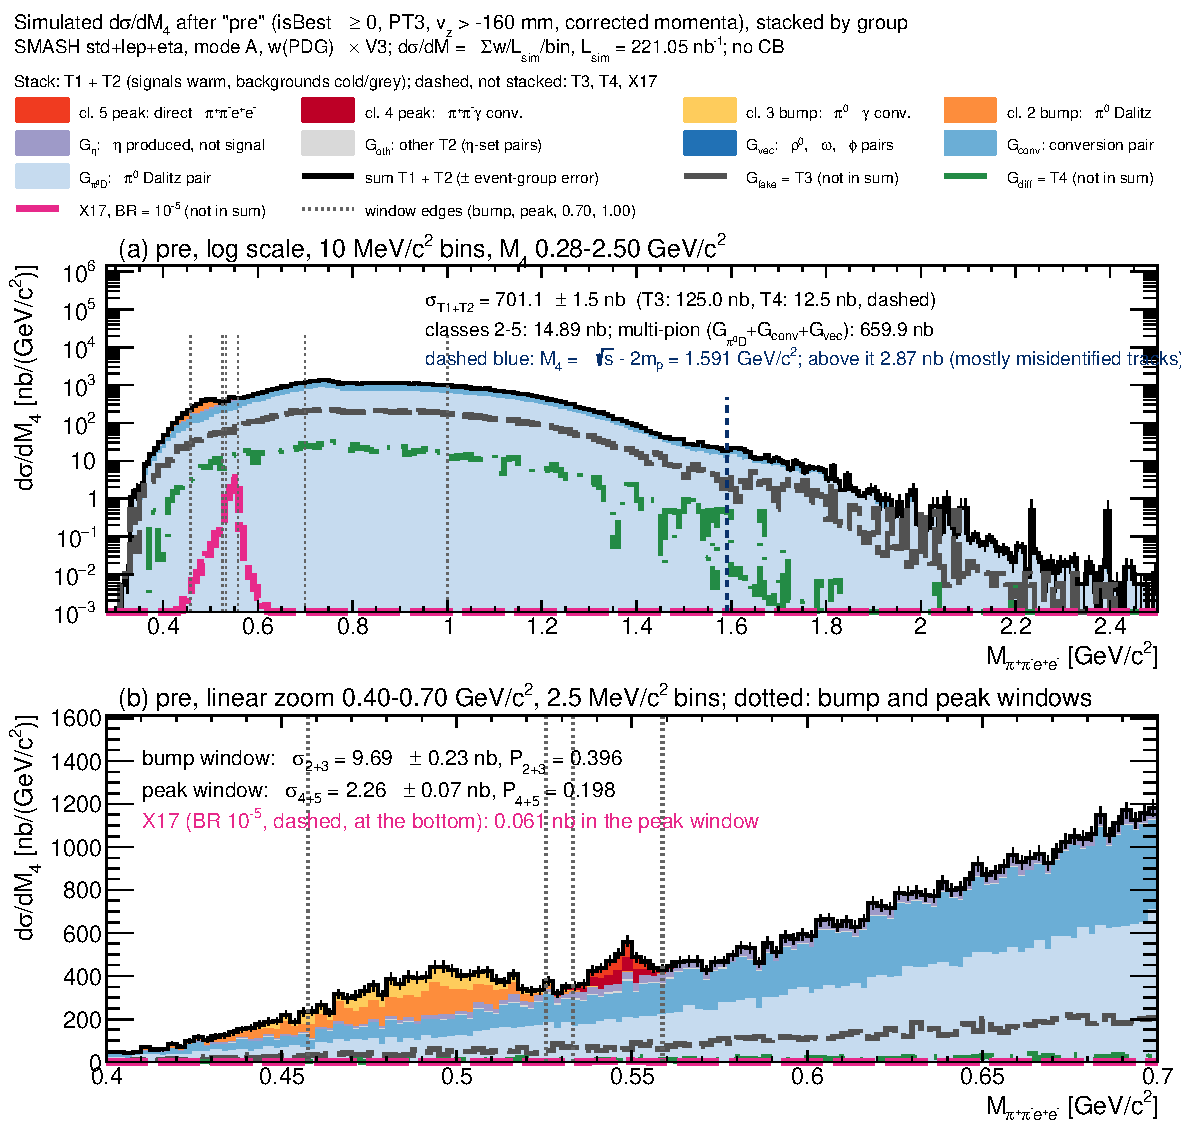
\includegraphics[width=\textwidth]{figs/s5_spec_full_pre.pdf}
\caption{Simulated $d\sigma/d\Mfour$ after ``pre'', stacked by group (signal classes warm,
background groups cold or grey). Dashed and not stacked: T3, T4 and X17 at
$\mathrm{BR} = 10^{-5}$. (a) Log scale, 10\,\MeVcc bins; the dashed blue line is the kinematic
limit. (b) Linear zoom, 2.5\,\MeVcc bins, with the bump and peak windows (dotted).}
\label{fig:s5full}
\end{figure}

\textbf{The cut sequence.} The four $\eta$-selection cuts of the analysis are applied one after
the other: $\mathrm{OA}>2^\circ$, $\alpha_{\mathrm{lab}}<50^\circ$, $\Mpipi<0.46$\,\GeVcc,
$\alpha_\eta>140^\circ$. All four together are the selection ``slides''.
Table~\ref{tab:s5flow} gives the cross sections, the purity $P$ = (signal in the window)/(T1+T2 in
the window) and $F = S/\sqrt{S+B}$, with $S$ the signal rows and $B$ the other T1+T2 rows of the
window at \Ldata. Figure~\ref{fig:s5steps} shows the spectrum after each step.

\begin{table}[H]
\centering
\caption{Cut sequence (nominal order). $\sigma$ in nb, errors from event groups. $P$: purity in
the window. $F = S/\sqrt{S+B}$ at $\Ldata = 6080.5\,\nbinv$ (UNCONFIRMED); in brackets $F$ with
$B$ + T3 + T4. Columns: the cuts OA$>2^\circ$, $\alpha_{\mathrm{lab}}<50^\circ$, $\Mpipi<0.46$\,\GeVcc and
$\alpha_\eta>140^\circ$ added one by one; last column: the final selection with $\Mpipi<0.42$\,\GeVcc.}
\label{tab:s5flow}
\footnotesize
\setlength{\tabcolsep}{3pt}
\begin{tabular}{@{}l rrrrr r@{}}
\toprule
 & pre & +OA & +$\alpha_{\mathrm{lab}}$ & +$M_{\pi\pi}$ & +$\alpha_\eta$ & $M_{\pi\pi}<0.42$ \\
\midrule
T1+T2, all $M_4$        & $701.1\pm1.5$ & $476.4\pm1.1$ & $254.0\pm0.9$ & $89.6\pm0.5$ & $67.9\pm0.5$ & $53.0\pm0.4$ \\
classes 2--5, all $M_4$ & $14.89\pm0.27$ & $10.58\pm0.22$ & $10.10\pm0.22$ & $10.06\pm0.22$ & $7.60\pm0.18$ & 7.26 \\
\midrule
bump: classes 2+3      & $9.69\pm0.23$ & $6.88\pm0.20$ & $6.61\pm0.19$ & $6.61\pm0.19$ & $5.60\pm0.17$ & $5.59\pm0.17$ \\
bump: T1+T2            & $24.48\pm0.33$ & $17.93\pm0.28$ & $16.71\pm0.27$ & $16.71\pm0.27$ & $15.08\pm0.25$ & $14.84\pm0.25$ \\
bump: $P$              & $0.396\pm0.007$ & $0.383\pm0.008$ & $0.395\pm0.008$ & $0.395\pm0.008$ & $0.371\pm0.008$ & $0.377\pm0.008$ \\
bump: $F$              & $152.7\pm3.0$ & $126.6\pm3.0$ & $126.0\pm3.0$ & $126.0\pm3.0$ & $112.5\pm2.9$ & $113.2\pm2.9$ \\
                       & (143.2) & (119.3) & (119.0) & (119.0) & (106.2) & (106.9) \\
\midrule
peak: classes 4+5      & $2.26\pm0.07$ & $1.57\pm0.05$ & $1.40\pm0.05$ & $1.37\pm0.05$ & $1.37\pm0.05$ & $1.07\pm0.04$ \\
peak: T1+T2            & $11.45\pm0.18$ & $8.45\pm0.15$ & $6.97\pm0.14$ & $6.79\pm0.13$ & $6.79\pm0.13$ & $5.64\pm0.12$ \\
peak: $P$              & $0.198\pm0.006$ & $0.185\pm0.006$ & $0.201\pm0.007$ & $0.202\pm0.007$ & $0.202\pm0.007$ & $0.190\pm0.007$ \\
peak: $F$              & $52.1\pm1.5$ & $42.0\pm1.3$ & $41.5\pm1.4$ & $41.0\pm1.4$ & $41.0\pm1.4$ & $35.3\pm1.2$ \\
                       & (48.1) & (39.0) & (38.4) & (38.0) & (38.0) & (32.6) \\
\bottomrule
\end{tabular}
\end{table}

\begin{figure}[H]
\centering
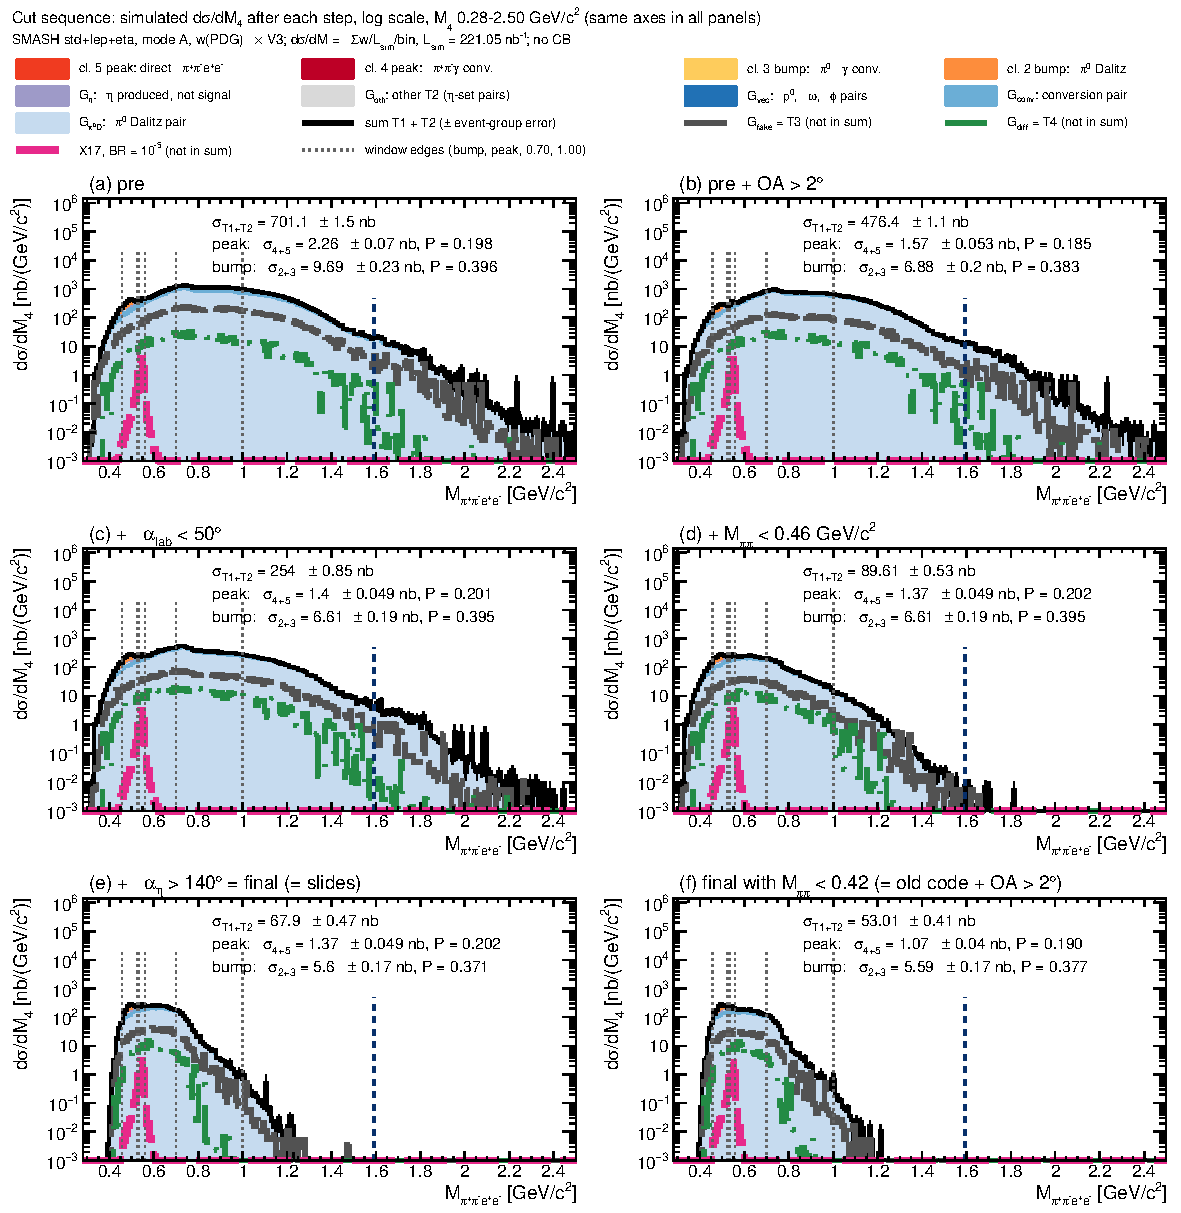
\includegraphics[width=\textwidth]{figs/s5_spec_steps_log.pdf}
\caption{Simulated $d\sigma/d\Mfour$ after each step of the cut sequence (same axes in all
panels; legend as in Fig.~\ref{fig:s5full}). (a) pre; (b)--(e) the four cuts added one by one;
(e) is ``slides''; (f) the final selection with $\Mpipi<0.42$\,\GeVcc.}
\label{fig:s5steps}
\end{figure}

\textbf{Where each cut acts.} Table~\ref{tab:s5where} gives, for each cut applied alone to
``pre'', the fraction of the background of each \Mfour region that it removes.
\begin{itemize}
\item OA$>2^\circ$ removes 25--36\,\% of the background in every region: it acts everywhere the same.
\item $\alpha_{\mathrm{lab}}$ and \Mpipi act mainly above the $\eta$: \Mpipi$<0.46$ removes
      nothing in the bump window, because there $\Mpipi\le\Mfour-\Mee$ is already below the
      limit, and 1.8\,\% in the peak window.
\item $\alpha_\eta$ is a band-pass in \Mfour. It is the angle between \pipi and \ee in a frame
      obtained by boosting with the measured total momentum and an energy computed with the
      $\eta$ mass (\code{Physics::}\allowbreak\code{openingAngleInMassConstrainedRestFrame}). For
      $\Mfour = m_\eta$ this frame is the true rest frame and the angle is exactly $180^\circ$. In
      the peak window the cut therefore removes nothing (efficiency 1.000 for every group); it
      removes 75\,\% of the background below the bump, 78\,\% in 0.70--1.00 and 99\,\% above
      1.00\,\GeVcc, and 10--14\,\% of the bump signal in the bump window.
\end{itemize}

\begin{table}[H]
\centering
\caption{Fraction of the background removed by each cut alone (from ``pre''). Background: T1+T2
minus the signal of the window in the bump and peak windows, T2 elsewhere. Errors 0.002--0.012
in the first three columns, below 0.002 elsewhere.}
\label{tab:s5where}
\footnotesize
\setlength{\tabcolsep}{4pt}
\begin{tabular}{@{}l rrrrrr r@{}}
\toprule
cut & $<0.4576$ & bump & peak & 0.56--0.70 & 0.70--1.00 & $>1.00$ & all \Mfour (T2) \\
\midrule
OA$>2^\circ$                     & 0.247 & 0.252 & 0.250 & 0.276 & 0.317 & 0.363 & 0.321 \\
$\alpha_{\mathrm{lab}}<50^\circ$ & 0.014 & 0.077 & 0.166 & 0.307 & 0.473 & 0.559 & 0.455 \\
$\Mpipi<0.46$\,\GeVcc            & 0.000 & 0.0005 & 0.018 & 0.254 & 0.631 & 0.876 & 0.616 \\
$\alpha_\eta>140^\circ$          & 0.751 & 0.053 & 0.000 & 0.075 & 0.781 & 0.987 & 0.702 \\
\bottomrule
\end{tabular}
\end{table}

\textbf{The order of the cuts matters for the attribution.} Inside the two windows the cuts
act almost independently: the fraction attributed to a cut changes by 10--20\,\% (relative)
between the nominal and the reverse order. Over the whole spectrum it changes completely:
$\alpha_\eta$ removes 69\,\% of T1+T2 when applied first, but 3\,\% when applied last. A
statement ``this cut removes that much background'' is therefore meaningful only per window and
together with the order.

\textbf{The resulting shape.} After ``slides'' the multi-pion background is still the largest
part of every window: 0.72 below the bump, 0.55 in the bump window, 0.70 in the peak window,
0.89 in 0.56--0.70\,\GeVcc. T1+T2 above 0.70\,\GeVcc drops from 545.9 to 9.96\,nb, from 78\,\% to
15\,\% of the spectrum. Above 1.00\,\GeVcc only 0.037\,nb remain, with $N_{\mathrm{eff}} = 33$.

\notebox{\textbf{Main result of the spectrum study.} In the simulation the four cuts do not
raise the purity of either window (bump $0.396\to0.371$, peak $0.198\to0.202$), and $F$ falls at
every step (peak $52.1\to41.0$, bump $152.7\to112.5$). What the cuts do is remove the multi-pion
background outside the windows. A gain from these cuts in data can only come from what the
simulation does not contain: the CB, or a data/SMASH difference of the multi-pion background.
This must be checked with data.}

%----------------------------------------------------------------------
\subsection{The signal at generator level}
\label{sec:s5gen}
%----------------------------------------------------------------------
\textbf{Number of produced decays.} The PLUTO generator file of the $\eta$ set holds the true
kinematics of $N = 1\,181\,801$ direct decays from 1000 of the 100\,000 files. Assuming these
files are representative, the set contains $N_{\mathrm{direct}} = 100\,N = 1.1818\times10^{8}$
direct decays. Every $\eta$ of the set is forced, half into the direct decay, so the set holds
$N_\eta = 2N_{\mathrm{direct}} = 2.364\times10^{8}$ $\eta$ mesons, i.e.
$\sigma(pp\to\eta X) = N_\eta/\Lsim = 1.069$\,mb in SMASH. The decays of the other channels
are $N_\eta$ times the PDG branching ratio (Table~\ref{tab:s5prod}). The statistical error of
this scale is 0.09\,\%; whether the 1000 files are representative is UNVERIFIED.

\begin{table}[H]
\centering
\caption{Produced decays per set ($10^{10}$ events) and production cross sections, from
$N_\eta$ and PDG branching ratios. Class 3 is counted per $\eta\to\pipi\piz$ decay with any \piz
decay (the conversion happens in the detector), class 4 per $\eta\to\pipi\gamma$ decay. Scale
error 0.09\,\% for every row.}
\label{tab:s5prod}
\small
\begin{tabular}{@{}l l r r@{}}
\toprule
Class & Channel & produced decays & $\sigma_{\mathrm{prod}}$ [nb] \\
\midrule
2 & $\eta\to\pipi\piz$, $\piz\to\ee\gamma$ & $6.360\times10^{5}$ & 2\,877.2 \\
3 & $\eta\to\pipi\piz$ (any \piz decay)     & $5.417\times10^{7}$ & 245\,075 \\
4 & $\eta\to\pipi\gamma$                    & $9.974\times10^{6}$ & 45\,123 \\
5 & $\eta\to\ppee$                          & $6.334\times10^{4}$ & 286.56 \\
6 & $\eta\to\pipi X17$, $X17\to\ee$, $\mathrm{BR}=10^{-5}$ & $2.364\times10^{3}$ & 10.693 \\
\bottomrule
\end{tabular}
\end{table}

\textbf{Shapes} (Fig.~\ref{fig:s5gen}). The physics weights replace the generator
distribution of the direct decay by Kroll--Wada $\times$ the P-wave rate $\times$ the form
factors $\times$ the decay angles (V3). The \Mee spectrum then becomes much harder:
\begin{center}
\small
\begin{tabular}{@{}l rrrrr@{}}
\toprule
fraction of produced decays with $\Mee >$ & 2 & 10 & 17 & 20 & 50\,\MeVcc \\
\midrule
direct, generator     & 0.513 & 0.099 & 0.057 & 0.047 & 0.016 \\
direct, V3            & 0.868 & 0.478 & 0.351 & 0.313 & 0.118 \\
bump \piz Dalitz (Kroll--Wada) & 0.860 & 0.443 & 0.308 & 0.268 & 0.070 \\
\bottomrule
\end{tabular}
\end{center}
The mean \Mpipi is 0.4007\,\GeVcc for the direct decay (V3), 0.3623 for the bump (KLOE-2; phase
space 0.3465), 0.4057 for the conversion peak ($|F_V|^2$; phase space 0.4014) and 0.3985 for X17
(three-body phase space, ASSUMED). The bump ends at $m_\eta-m_{\piz} = 0.413$\,\GeVcc.

\textbf{Direct decays under the X17 line.} The direct decay has a continuous \Mee spectrum and
contributes under any X17 line. With V3, the produced direct decays within $|\Mee-17| < d$ are
4.04, 7.95, 15.9 and 32.4\,nb for $d = 0.5$, 1, 2 and 4\,\MeVcc; X17 with
$\mathrm{BR}=10^{-5}$ is 10.69\,nb (Fig.~\ref{fig:s5gen}d).

\begin{figure}[H]
\centering
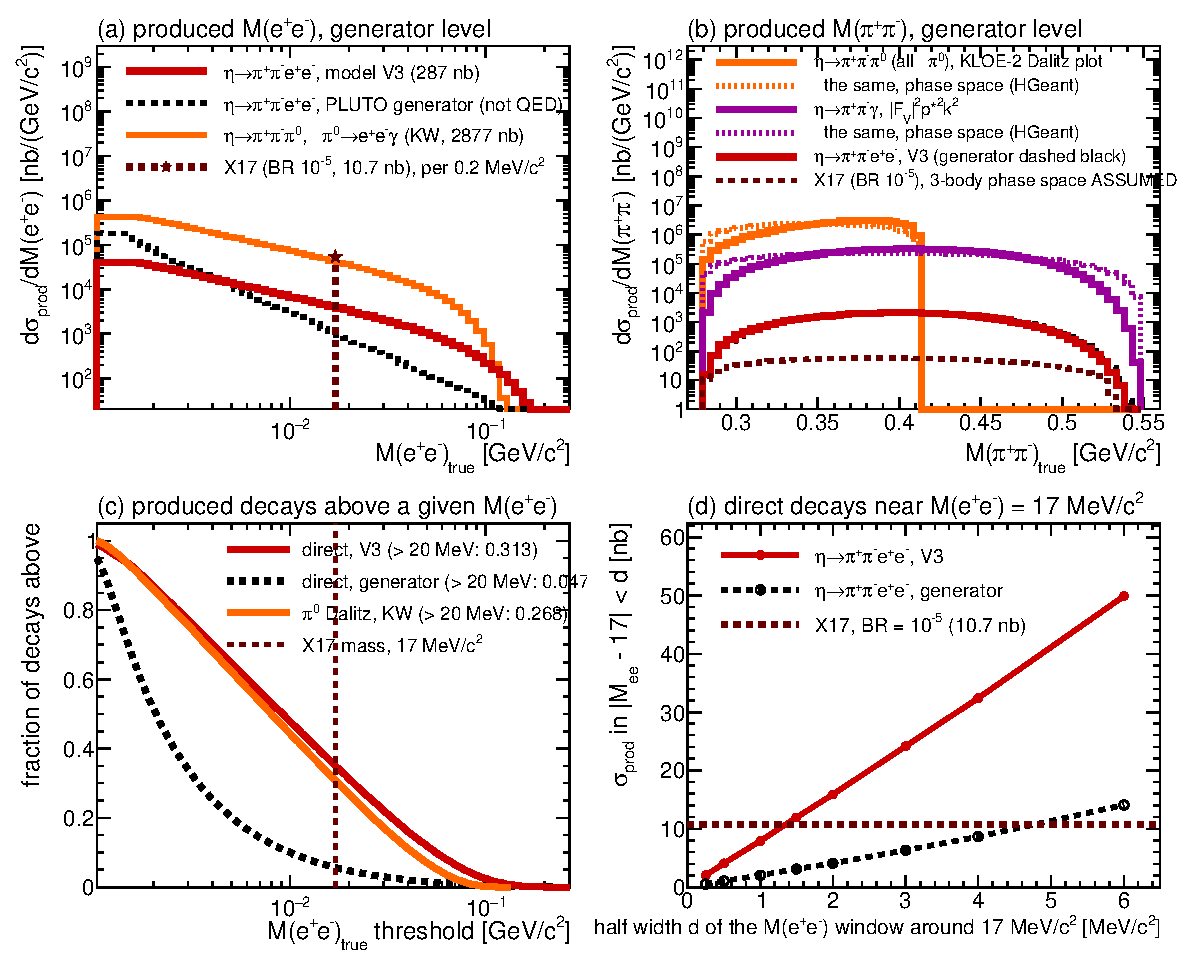
\includegraphics[width=\textwidth]{figs/s5_acc_gen.pdf}
\caption{Generator level, absolute scale ($\sigma_{\mathrm{prod}}$). (a) \Mee of the direct decay
(V3 and generator), of the \piz Dalitz pair of the bump, and the X17 line. (b) \Mpipi of all
channels: physics models (solid) against the phase space of HGeant (dotted). (c) Fraction of
decays above a given \Mee. (d) Direct decays in a window $\pm d$ around 17\,\MeVcc against X17 at
$\mathrm{BR}=10^{-5}$.}
\label{fig:s5gen}
\end{figure}

%----------------------------------------------------------------------
\subsection{Acceptance and resolution}
\label{sec:s5acc}
%----------------------------------------------------------------------
\textbf{Acceptance $\times$ efficiency} $\varepsilon$ = (rows of the class after ``pre'', weighted)
/ (produced decays). Every accepted decay gives exactly one row of its class.
Table~\ref{tab:s5eps} gives the totals.

\begin{table}[H]
\centering
\caption{Acceptance $\times$ efficiency of ``pre'' per produced decay, in \%. Classes 3 and 4
include the conversion probability (per $\eta\to\pipi\piz$ and per $\eta\to\pipi\gamma$ decay).
X17: at $\mathrm{BR}=10^{-5}$.}
\label{tab:s5eps}
\footnotesize
\setlength{\tabcolsep}{4pt}
\begin{tabular}{@{}l rr r rr rr@{}}
\toprule
 & & & & \multicolumn{2}{c}{$\varepsilon$, all $M_4$} & \multicolumn{2}{c}{$\varepsilon$ (V3), window} \\
class & rows & $N_{\mathrm{eff}}$ & $\sigma_{\mathrm{acc}}$ [nb] & V3 & no weights & peak & bump \\
\midrule
5 direct    & 571\,246 & 171\,004 & $1.4168\pm0.0034$ & $0.4944\pm0.0013$ & 0.4834 & 0.4213 & 0.0249 \\
6 X17       & 787\,659 & 787\,653 & 0.0713 & $0.6665\pm0.0010$ & 0.6665 & 0.5714 & 0.0352 \\
2 bump Dalitz & 1\,649 & 1\,332 & $7.05\pm0.19$ & $0.245\pm0.007$ & 0.275 & 0.0010 & 0.194 \\
3 bump conv.  & 1\,187 &   948 & $5.19\pm0.17$ & $0.00212\pm0.00007$ & 0.00238 & 0 & 0.00167 \\
4 peak conv.  &   307 &   270 & $1.24\pm0.08$ & $0.00275\pm0.00017$ & 0.00272 & 0.00234 & 0.00013 \\
\bottomrule
\end{tabular}
\end{table}

Figure~\ref{fig:s5acc} shows $\varepsilon$ against the true \Mee and \Mpipi.
\begin{itemize}
\item \textbf{True \Mee} (direct decay, V3): 0.34--0.37\,\% at 2--4\,\MeVcc, 0.49\,\% at 10, 0.53\,\% at
      16--20, 0.58\,\% at 45--57, 0.96\,\% at 100--124 and 1.8--2.0\,\% above 160\,\MeVcc. A pair of
      small mass has a small opening angle and is often lost. The two lowest bins are affected by
      the stored precision of the generator file.
\item \textbf{Decay angles.} At fixed \Mee, V3 lowers $\varepsilon$ by the factor 0.82 at
      5--20\,\MeVcc and 0.84--0.90 at 20--75\,\MeVcc (Fig.~\ref{fig:s5acc}c). The cause is the QED
      $e^+$ angle $1+\cos^2\theta^*_e$: V2, the same model without the angles, changes $\varepsilon$
      by less than 6\,\%. Over all \Mee V3 still raises $\varepsilon$ by 2.3\,\%, because it moves
      decays to higher \Mee.
\item \textbf{True \Mpipi.} $\varepsilon$ falls steeply with \Mpipi, because a heavy pion pair leaves
      slow leptons: direct decay 0.86\,\% at 0.29--0.30, 0.47\,\% at 0.41--0.42, 0.016\,\% at
      0.49--0.50 and 0 above 0.52\,\GeVcc.
\item \textbf{X17 against the direct decay} at the same true \Mee (14--20\,\MeVcc): without physics
      weights the two agree within about 5\,\% below $\Mpipi = 0.45$\,\GeVcc (Fig.~\ref{fig:s5acc}d).
      This supports, but does not prove, the phase-space \Mpipi and the isotropic decay assumed
      for X17.
\end{itemize}

\begin{figure}[H]
\centering
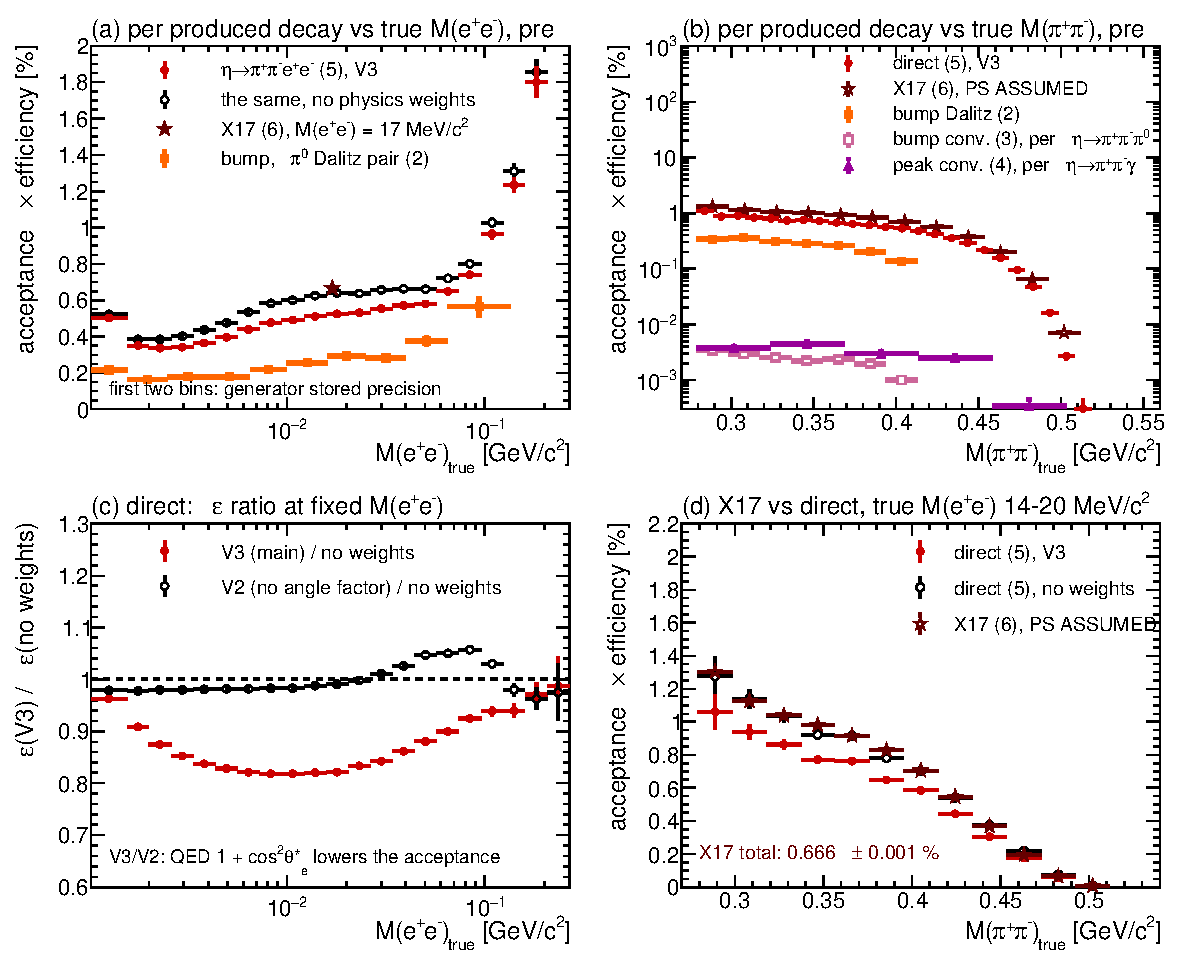
\includegraphics[width=\textwidth]{figs/s5_acc_eff_mass.pdf}
\caption{Acceptance $\times$ efficiency of ``pre'' per produced decay. (a) Against the true \Mee:
direct decay (V3 and without physics weights), bump \piz Dalitz pair, X17. (b) Against the true
\Mpipi for all classes. (c) Ratio V3/no weights and V2/no weights at fixed \Mee: the effect of the
decay angles. (d) X17 against the direct decay at true \Mee 14--20\,\MeVcc.}
\label{fig:s5acc}
\end{figure}

\textbf{Resolution and scale} (Table~\ref{tab:s5res}, Fig.~\ref{fig:s5res}). The difference
reconstructed minus true is fitted with a Gaussian core (iterated in $\pm2\sigma$); the tails are
counted outside $\pm3\sigma$. The reconstructed \Mfour is low by 0.25--0.39\,\% (median ratio)
and has a low-side tail from energy loss and radiation: 6\,\% of the direct decays lie more than
$3\sigma$ below the core. The \Mee resolution comes from the opening-angle measurement (OA
resolution 1.0--1.4$^\circ$): at 17\,\MeVcc the core width is $4.21\pm0.01$\,\MeVcc with a median
shift of $+0.10$\,\MeVcc; 90\,\% of the X17 rows lie in 9.7--24.3\,\MeVcc.

\begin{table}[H]
\centering
\caption{Resolution of \Mfour (reconstructed with corrected momenta minus true), after ``pre''.}
\label{tab:s5res}
\footnotesize
\setlength{\tabcolsep}{4pt}
\begin{tabular}{@{}l rr c r r@{}}
\toprule
 & \multicolumn{2}{c}{$\Delta M_4$ [\MeVcc]} & tail fraction & median & $\Delta M_{\pi\pi}$ core \\
class & median & core $\sigma$ & below / above $3\sigma$ & $M_4/M_{4,\mathrm{true}}$ & $\sigma$ [\MeVcc] \\
\midrule
5 direct      & $-2.12\pm0.02$ & $6.44\pm0.02$ & 0.057 / 0.014 & 0.99614 & $3.49\pm0.01$ \\
6 X17         & $-2.10\pm0.01$ & $6.25\pm0.01$ & 0.063 / 0.013 & 0.99617 & $2.98\pm0.01$ \\
2 bump Dalitz & $-1.47\pm0.22$ & $5.47\pm0.18$ & 0.041 / 0.015 & 0.99694 & $3.13\pm0.12$ \\
3 bump conv.  & $-1.05\pm0.27$ & $5.68\pm0.26$ & 0.033 / 0.020 & 0.99783 & $3.11\pm0.13$ \\
4 peak conv.  & $-1.33\pm0.57$ & $6.13\pm0.40$ & 0.060 / 0.008 & 0.99757 & $3.15\pm0.26$ \\
\bottomrule
\end{tabular}
\end{table}

\begin{figure}[H]
\centering
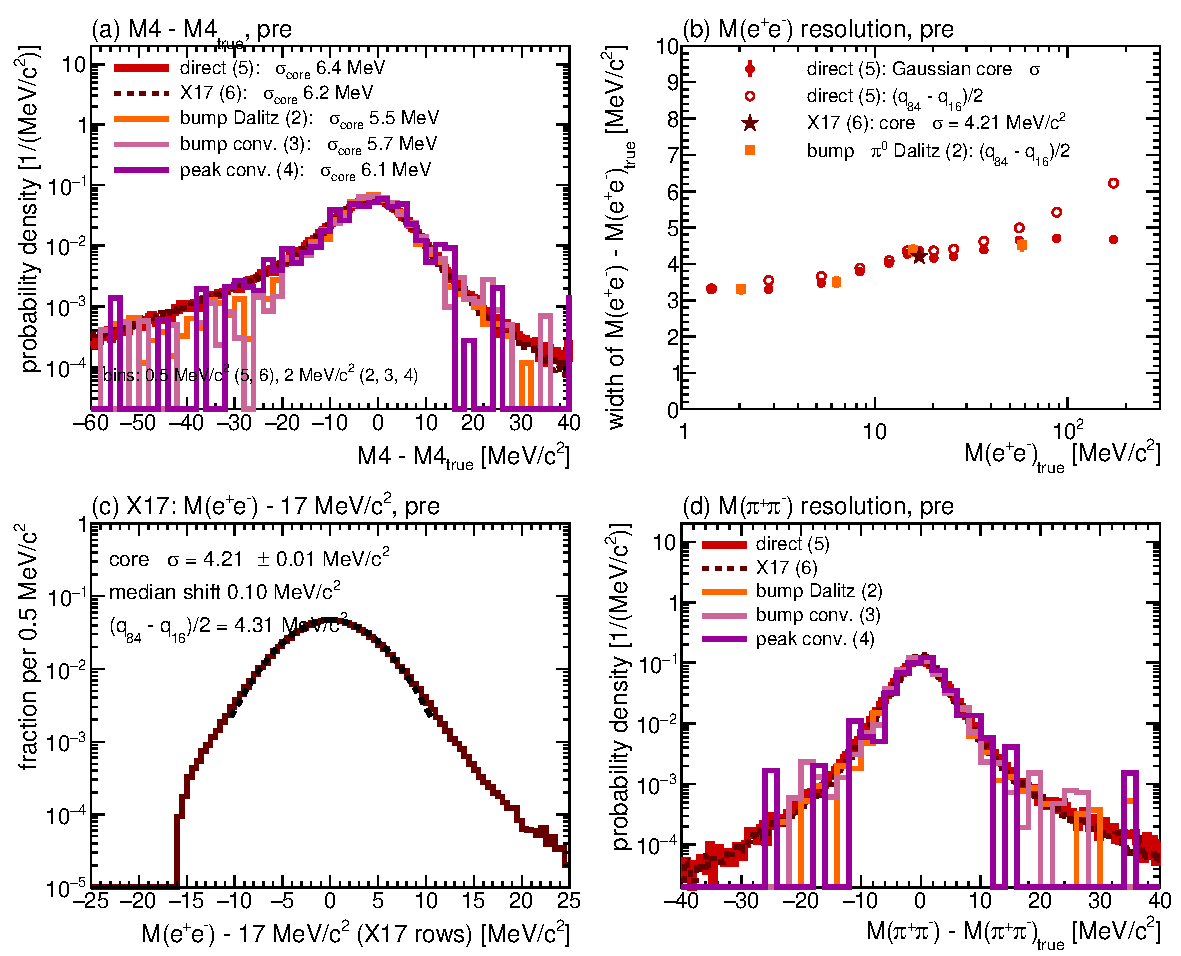
\includegraphics[width=\textwidth]{figs/s5_acc_res.pdf}
\caption{Resolution after ``pre''. (a) $\Mfour-M_{4,\mathrm{true}}$ per class. (b) Width of
$\Mee-M_{ee,\mathrm{true}}$ against the true \Mee. (c) Reconstructed \Mee of the X17 rows minus
17\,\MeVcc. (d) $\Mpipi-M_{\pi\pi,\mathrm{true}}$.}
\label{fig:s5res}
\end{figure}

\textbf{Check of the peak window.} A Gaussian fit of the simulated peak (classes 4+5, V3, 1\,\MeVcc
bins, iterated in $\pm2\sigma$) gives $\mu = 0.54637\pm0.00020$\,\GeVcc and
$\sigma = 6.09\pm0.19$\,\MeVcc, so $\mu\pm1.9\sigma$ = 0.5348--0.5579\,\GeVcc. The fixed window
(0.5333--0.5587) is 1.5\,\MeVcc wider on the low side. Nine fit choices (bin width, fit range)
move the lower edge by $+0.1$ to $+3.2$\,\MeVcc; the direct decay alone ($N_{\mathrm{eff}}$ 171\,000)
reproduces the fixed window within 0.7\,\MeVcc. The fixed window is therefore kept. It holds 0.851
of the simulated peak, $2.262\pm0.070$\,nb (direct $1.207\pm0.003$, conversion $1.054\pm0.070$).

\textbf{The opening angle separates conversions only weakly.} The true OA of a conversion pair is
small (median 0.51$^\circ$), but the reconstructed OA is larger by about 1.6$^\circ$ (median
2.2$^\circ$), because of the OA resolution and the need for two separated tracks. The fraction with
OA$>2^\circ$ is 0.811 (direct), 0.955 (X17), $0.814\pm0.011$ (bump Dalitz), $0.576\pm0.016$ (bump
conversion) and $0.567\pm0.030$ (peak conversion). A cut on \Mee separates about as well:
$\Mee>15$\,\MeVcc keeps 0.50 of the direct decay and 0.02 of the conversion peak.
OA does not separate X17 from the direct decay at the same reconstructed \Mee.

%----------------------------------------------------------------------
\subsection{Cut flow per signal class and background composition}
\label{sec:s5cut}
%----------------------------------------------------------------------
Eight cuts are studied: the four of ``slides'', both pions in the vertex fit,
$\max|z_\pi-z_{\mathrm{vertex}}|<40$\,mm (written $|\Delta z_\pi|$), $\mathrm{MM}_4<2.85$\,\GeVcc and
$p_{T,4}>400$\,\MeVc. For each cut we compute the efficiency $\varepsilon_S$ of the signal and
$\varepsilon_B$ of the background T2 in a window, and
\begin{equation}
Q = \varepsilon_S/\sqrt{\varepsilon_B}.
\end{equation}
$Q$ is the factor by which the cut changes $S/\sqrt{B}$ when $B\gg S$; it needs no luminosity. A cut
carries information if $Q > 1 + \max(0.02, 2\delta Q)$ and is harmful if $Q$ is below the mirror
value. ``Alone'' means the cut on ``pre''; ``N$-$1'' means the cut on top of the other three slides
cuts (for the four other cuts: on top of ``slides''). Errors are from event groups, with pass and
fail rows of one event correlated.

\begin{table}[H]
\centering
\caption{Efficiencies and $Q$ of each cut alone (from ``pre'') in the windows. Peak: $S$ = classes
4+5; bump: $S$ = classes 2+3; X17: $S$ = X17, $B$ = T2 + classes 4+5 (peak window). The error is
in brackets, in units of the last digit.}
\label{tab:s5rank}
\footnotesize
\setlength{\tabcolsep}{3pt}
\begin{tabular}{@{}l ccc ccc cc@{}}
\toprule
 & \multicolumn{3}{c}{peak window} & \multicolumn{3}{c}{bump window} & \multicolumn{2}{c}{X17 (peak window)} \\
cut & $\varepsilon_S$ & $\varepsilon_B$ & $Q$ & $\varepsilon_S$ & $\varepsilon_B$ & $Q$ & $\varepsilon_S$ & $Q$ \\
\midrule
OA$>2^\circ$                     & 0.693(16) & 0.749(8) & 0.801(19) & 0.710(11) & 0.748(7) & 0.820(13) & 0.957 & 1.114(6) \\
$\alpha_{\mathrm{lab}}<50^\circ$ & 0.916(9) & 0.834(7) & 1.003(10) & 0.970(3) & 0.922(4) & 1.010(4) & 0.892 & 0.967(3) \\
$\Mpipi<0.46$                    & 0.981(4) & 0.982(2) & 0.990(4) & 1.000 & 1.000 & 1.000 & 0.980 & 0.989(1) \\
$\alpha_\eta>140^\circ$          & 1.000 & 1.000 & 1.000 & 0.858(10) & 0.947(3) & 0.882(10) & 1.000 & 1.000 \\
pions in vertex fit              & 0.938(7) & 0.806(7) & 1.045(9) & 0.923(6) & 0.784(6) & 1.042(8) & 0.931 & 1.020(4) \\
$|\Delta z_\pi|<40$\,mm          & 0.963(5) & 0.829(7) & 1.058(7) & 0.944(6) & 0.813(6) & 1.047(7) & 0.962 & 1.040(3) \\
$\mathrm{MM}_4<2.85$             & 0.963(5) & 0.904(6) & 1.013(7) & 0.949(5) & 0.886(5) & 1.008(6) & 0.963 & 1.007(3) \\
$p_{T,4}>400$\,\MeVc             & 0.795(12) & 0.588(9) & 1.037(18) & 0.849(8) & 0.712(7) & 1.006(11) & 0.791 & 0.998(6) \\
\midrule
slides (all four), from pre      & 0.606(16) & & 0.790(22) & 0.578(12) & & 0.722(15) & & 1.077(7) \\
\bottomrule
\end{tabular}
\end{table}

What the numbers say (Table~\ref{tab:s5rank}, Figs.~\ref{fig:s5regions} and~\ref{fig:s5rank}):
\begin{itemize}
\item \textbf{Inside the windows the cuts hardly separate signal from the simulated background.}
      Only the two pion-vertex cuts have $Q>1$ significantly ($Q$ = 1.04--1.06 in both windows).
      They select the same rows: given all other cuts, each adds nothing ($Q$ = 0.99--1.02).
      Signal pions come from the primary vertex; 9--15\,\% of the background pion pairs contain a
      $\pi\to\mu$ decay and 28--32\,\% secondary pions.
\item \textbf{OA$>2^\circ$ is harmful for the $\eta$ windows} ($Q = 0.80$ peak, 0.82 bump): it
      removes the signal conversions (classes 3 and 4 keep 0.56--0.57) at the same rate as the
      background conversions. It is informative only for X17 ($Q = 1.114\pm0.006$), whose pairs have a
      median OA of 4.6$^\circ$ against 2.1--2.2$^\circ$ for conversions.
\item \textbf{$\alpha_\eta>140^\circ$} does nothing in the peak window and costs bump signal
      ($Q = 0.882\pm0.010$): it keeps 0.86 of the bump and 0.95 of T2.
\item \textbf{The slides cuts are an \Mfour band-pass} (Fig.~\ref{fig:s5regions}): T2 kept by
      ``slides'' is 0.17 below the bump, 0.64 in the bump window, 0.59 in the peak window, 0.30 in
      0.56--0.70, 0.029 in 0.70--1.00 and $1.8\times10^{-4}$ above 1.00\,\GeVcc. Inside the windows
      they cost 39\,\% (peak) and 42\,\% (bump) of the signal. Their value is a cleaner spectrum
      around the $\eta$ (fits, side bands) and, in data, possibly a smaller CB; neither can be measured
      in this simulation.
\end{itemize}

\begin{figure}[H]
\centering
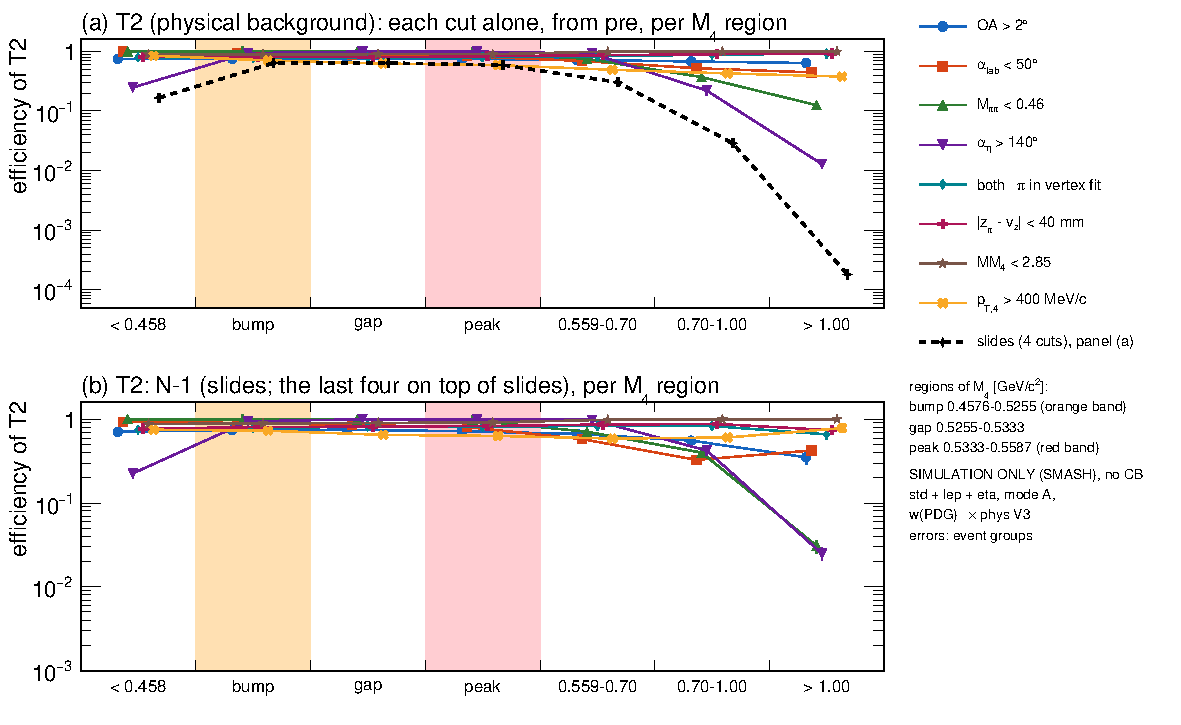
\includegraphics[width=\textwidth]{figs/s5_cut_regions.pdf}
\caption{Efficiency of the physical background T2 per \Mfour region. (a) Each cut alone on
``pre'', and the four slides cuts together (dashed). (b) N$-$1: each cut on top of the other
slides cuts (the last four cuts on top of ``slides''). Errors from event groups.}
\label{fig:s5regions}
\end{figure}

\begin{figure}[H]
\centering
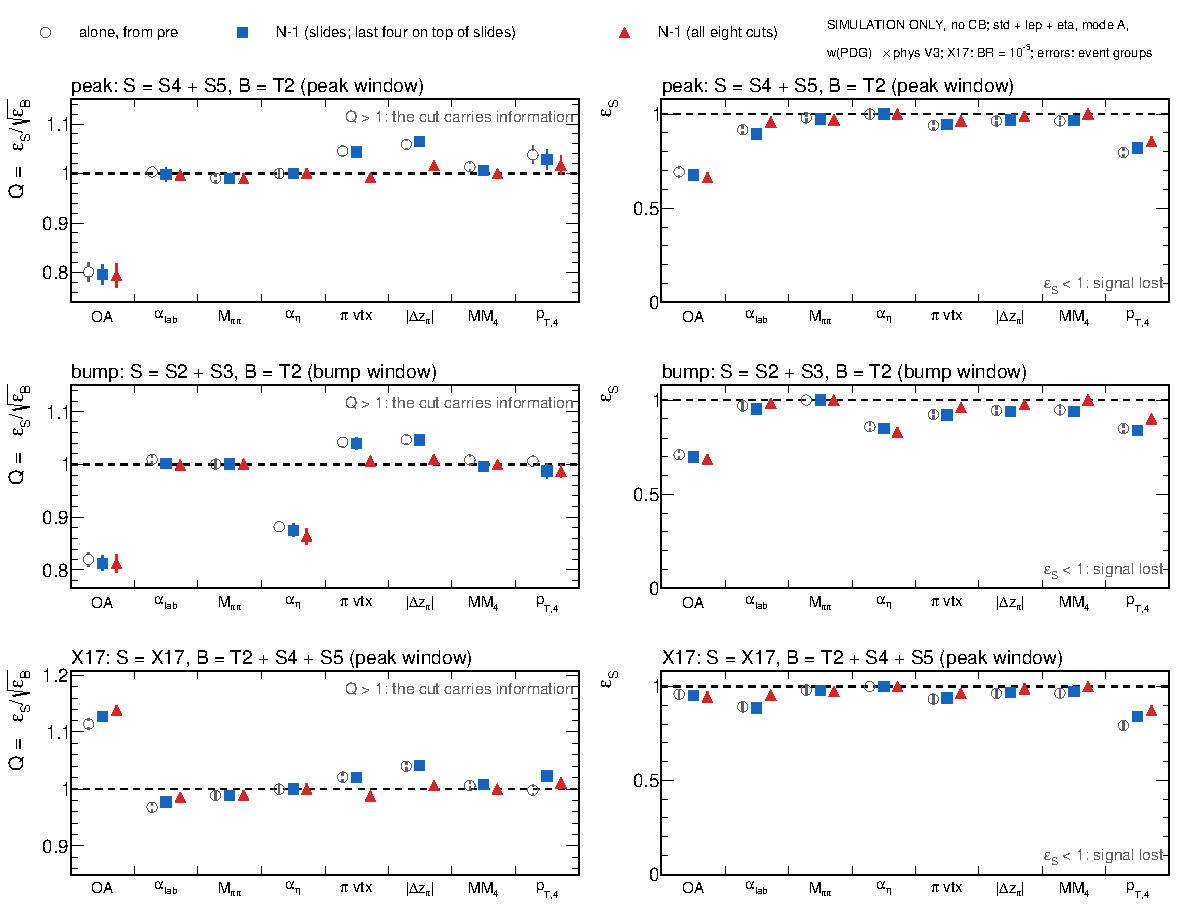
\includegraphics[width=\textwidth]{figs/s5_cut_rank.pdf}
\caption{$Q = \varepsilon_S/\sqrt{\varepsilon_B}$ (left) and $\varepsilon_S$ (right) of the eight cuts
for the peak, the bump and X17 ($\mathrm{BR}=10^{-5}$): alone (open circles), N$-$1 with respect
to ``slides'' (squares), N$-$1 with respect to all eight cuts (triangles).}
\label{fig:s5rank}
\end{figure}

\textbf{Background composition} (Table~\ref{tab:s5comp}). The physical background has the same
make-up in every \Mfour region: \piz Dalitz pairs (L1, 53--60\,\% of T2) and conversion pairs (L3,
28--39\,\%). The pions are mostly both primary (P7, 40--72\,\%) or mixed/secondary (P8, 13--33\,\%);
9--15\,\% of the pion pairs contain a $\pi\to\mu$ decay (P1). $G_\eta$ is 7--10\,\% of T2 around the
$\eta$ and $G_{\mathrm{vec}}$ is negligible. T3 (not in the sum) is 12--20\,\% of T1+T2 near the
$\eta$; 60\,\% of T3 in the peak window are conversion pairs.

\begin{table}[H]
\centering
\caption{Composition after ``pre'' per \Mfour region: $\sigma$ of T1+T2, share of the signal
classes in T1+T2, shares of the groups in T2, and T3, T4 relative to T1+T2 (not in the sum).}
\label{tab:s5comp}
\small
\begin{tabular}{@{}l r r rrr rr@{}}
\toprule
region [\GeVcc] & T1+T2 [nb] & signal share & $G_\eta$ & $G_{\pi^0\mathrm{D}}$ & $G_{\mathrm{conv}}$ & T3 & T4 \\
\midrule
$<0.4576$    & $7.66\pm0.17$ & 0.310(11) & 0.067 & 0.539 & 0.384 & 0.147 & 0.012 \\
bump         & $24.48\pm0.33$ & 0.401(7) & 0.082 & 0.539 & 0.365 & 0.119 & 0.019 \\
gap          & $2.67\pm0.09$ & 0.100(10) & 0.078 & 0.535 & 0.369 & 0.202 & 0.028 \\
peak         & $11.45\pm0.18$ & 0.201(6) & 0.093 & 0.527 & 0.364 & 0.150 & 0.025 \\
0.5587--0.70 & $109.0\pm0.6$ & 0.0013(2) & 0.064 & 0.554 & 0.377 & 0.186 & 0.024 \\
0.70--1.00   & $340.9\pm1.0$ & $<10^{-4}$ & 0.033 & 0.573 & 0.392 & 0.179 & 0.018 \\
$>1.00$      & $205.0\pm0.7$ & 0 & 0.017 & 0.595 & 0.387 & 0.183 & 0.014 \\
\bottomrule
\end{tabular}
\end{table}

\textbf{Statistics.} The std-set signal classes limit every number of this part. In the windows
after ``pre'' class~2 has $N_{\mathrm{eff}} = 1022$, class~3 718 and class~4 225; after all eight
cuts 526, 268 and 79. $G_{\mathrm{vec}}$ and $G_{\mathrm{diff}}$ have $N_{\mathrm{eff}}$ below 150.

%----------------------------------------------------------------------
\subsection{Optimisation for the \texorpdfstring{$\eta$}{eta} peak and bump}
\label{sec:s5opt}
%----------------------------------------------------------------------
\textbf{Targets.} PEAK: classes 4+5 in the peak window. DIRECT: class 5 in the peak window, with
class~4 counted as background. BUMP: classes 2+3 in the bump window. $B$ = all other T1+T2 rows of
the window; a variant adds T3 and T4.

\textbf{Figure of merit and method.} $F = S/\sqrt{S+B}$ with $S$, $B$ in expected rows at
$\Ldata$ (UNCONFIRMED; $F\propto\sqrt{\Ldata}$, the position of the optimum does not depend on it).
Nine cut variables are scanned on grids that contain every named selection: OA$>$ (10 values),
$\alpha_{\mathrm{lab}}<$ (10), $\Mpipi>$ (9), $\Mpipi<$ (10), $\alpha_\eta>$ (8), pions in the
vertex fit (off/on), $|\Delta z_\pi|<40$\,mm (off/on), $\mathrm{MM}_4<$ (8) and $p_{T,4}>$ (6),
$13\,824\,000$ combinations in all. Each window row gets a grid index per variable; the weights are
filled into a 9-dimensional histogram and summed cumulatively along every axis. After that each
cell holds the exact $S$ and $B$ of one combination, and every cell is evaluated (exhaustive
search, no random sampling). The table reproduces the engine sums for all named selections and
direct row loops for 30 random cells (relative difference $<10^{-9}$; 378 checks).

\textbf{Freeze rule} (declared before the search). A candidate must reach $F\ge0.95\,F_{\mathrm{best}}$ on
the full sample and on each half (relative to the best of that half). Among the candidates take
the one with the fewest active cuts, then the one whose worst grid neighbour (each active
threshold moved by one step) has the highest $F$.

\begin{table}[H]
\centering
\caption{Optimisation of the $\eta$ selection (full sample, $\Ldata = 6080.5\,\nbinv$
UNCONFIRMED; errors: simulation statistics). $|\Delta z_\pi|$ stands for $\max|z_\pi-z_{\mathrm{vertex}}|<40$\,mm.
The last two rows are differences of $F$ with the event-group error computed on the difference
itself: the same rows enter both selections, so this error is much smaller than the errors of the
two $F$.}
\label{tab:s5opt}
\small
\begin{tabularx}{\textwidth}{@{}>{\raggedright\arraybackslash}p{3.6cm} L L L@{}}
\toprule
 & PEAK & DIRECT & BUMP \\
\midrule
$F$ at ``pre'' (purity) & $52.12\pm1.51$ (0.198) & $27.83\pm0.23$ (0.105) & $152.7\pm3.0$ (0.396) \\
best cell & $\Mpipi$ 0.32--0.48, $\alpha_\eta>160^\circ$, $|\Delta z_\pi|$, $\mathrm{MM}_4<2.85$
          & $\Mpipi$ 0.30--0.53, $\alpha_\eta>150^\circ$, $|\Delta z_\pi|$, $\mathrm{MM}_4<2.85$
          & $\alpha_{\mathrm{lab}}<70^\circ$, $\Mpipi$ 0.30--0.41, $|\Delta z_\pi|$ \\
$F$ of the best cell (purity) & $56.18\pm1.74$ (0.262) & $29.50\pm0.28$ (0.130) & $157.0\pm3.2$ (0.467) \\
frozen cut & $|\Delta z_\pi|<40$\,mm, $\mathrm{MM}_4<2.85$ & $|\Delta z_\pi|<40$\,mm & none (= pre) \\
$F$ frozen ($F/F_{\mathrm{best}}$) & $54.79\pm1.63$ (0.975) & $28.95\pm0.26$ (0.982) & $152.7\pm3.0$ (0.973) \\
purity, efficiency (frozen) & $0.234\pm0.007$, $0.931\pm0.007$ & $0.119\pm0.002$, $0.963\pm0.001$ & $0.396\pm0.007$, 1 \\
$F$(frozen) $-$ $F$(pre) & $+2.67\pm0.44$ & $+1.12\pm0.10$ & 0 \\
$F$(frozen) $-$ $F$(pre + pions in vertex fit) & $+1.19\pm0.48$ & $+0.58\pm0.09$ & $-1.11\pm0.88$ \\
\bottomrule
\end{tabularx}
\end{table}

\textbf{Results} (Table~\ref{tab:s5opt}, Figs.~\ref{fig:s5profile} and~\ref{fig:s5optcomp}).
\begin{itemize}
\item \textbf{The surface of $F$ is flat.} The plateau ($F\ge0.95\,F_{\mathrm{best}}$) contains, for PEAK:
      OA none or $>1^\circ$; $\alpha_{\mathrm{lab}}<40^\circ$ or looser; $\Mpipi>$ none to 0.34;
      $\Mpipi<0.46$ or looser; any $\alpha_\eta$ up to 170$^\circ$; $\mathrm{MM}_4<2.7$ or looser;
      $p_{T,4}>400$ or looser. The other targets are similar.
\item \textbf{The frozen cuts are better than ``pre'', but only a little.} With the correlated
      error the gain is significant in the simulation: $+2.67\pm0.44$ (5.1\,\%) for PEAK and
      $+1.12\pm0.10$ (4.0\,\%) for DIRECT. Compared with ``pre + pions in vertex fit'' the frozen
      cuts gain $+1.19\pm0.48$ (PEAK) and $+0.58\pm0.09$ (DIRECT). For BUMP no cut is frozen; the
      best cell gains $+4.3\pm1.0$, but this includes the optimisation bias (below).
\item \textbf{The PEAK choice was a knife edge.} ``$|\Delta z_\pi|<40$\,mm'' alone reaches 0.966 of
      $F_{\mathrm{best}}$ on the full sample but 0.9494 on half~B: it missed the half condition by
      0.0006, and the rule added $\mathrm{MM}_4<2.85$ (+1\,\% in $F$). On random halves the rule picks
      ``$|\Delta z_\pi|<40$\,mm'' alone in 167 of 200 cases.
\item \textbf{OA$>2^\circ$ is off the plateau for all three targets}, even for DIRECT, where it keeps
      only 0.81 of the direct decay. Only ``pions in vertex fit'', ``peak nominal'' and (for BUMP)
      ``bump nominal'' are on the plateau (Table~\ref{tab:s5presets}).
\item \textbf{Purity.} The cuts can raise the purity at a small loss of $F$: for BUMP, ``bump
      nominal'' gives 0.456 and the best purity on the plateau ($\alpha_{\mathrm{lab}}<40^\circ$,
      $\Mpipi>0.32$, $|\Delta z_\pi|$) 0.496, against 0.396 at ``pre''. These purity choices are not
      stable between halves (the most frequent half pick occurs in only 32--61 of 200 cases).
\end{itemize}

\begin{table}[H]
\centering
\caption{Named selections: $F/F_{\mathrm{best}}$ per target (errors about 3\,\% PEAK, 1\,\% DIRECT,
2\,\% BUMP; $\Ldata$ UNCONFIRMED).}
\label{tab:s5presets}
\small
\begin{tabular}{@{}l ccc@{}}
\toprule
selection & PEAK & DIRECT & BUMP \\
\midrule
pre                     & 0.928 & 0.943 & 0.973 \\
pre + OA$>2^\circ$       & 0.748 & 0.889 & 0.806 \\
pre + pions in vertex fit & 0.954 & 0.962 & 0.980 \\
slides                  & 0.730 & 0.889 & 0.716 \\
old code                & 0.784 & 0.848 & 0.877 \\
peak nominal            & 0.941 & 0.953 & 0.979 \\
bump nominal            & 0.732 & 0.783 & 0.977 \\
\bottomrule
\end{tabular}
\end{table}

\begin{figure}[H]
\centering
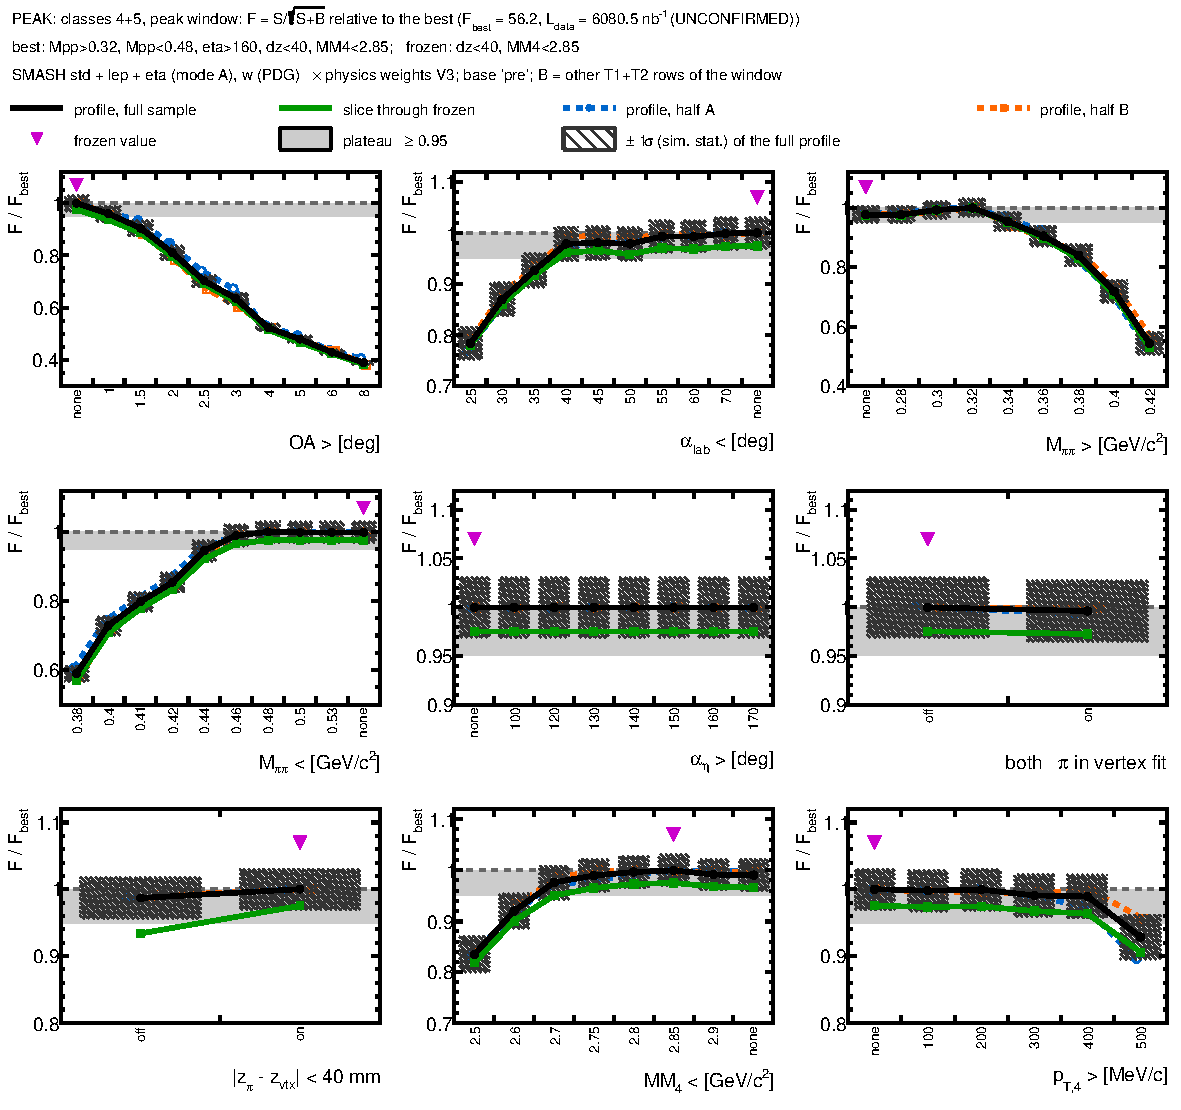
\includegraphics[width=\textwidth]{figs/s5_opt_eta_profile_peak.pdf}
\caption{PEAK target: $F/F_{\mathrm{best}}$ against each cut variable. Profile = the best $F$ over
all other variables at a fixed value (full sample, black; half A and half B relative to their
own best, dashed). The hatched band is the $\pm1\sigma$ statistical error of the full-sample $F$
at each profile point; differences between neighbouring points are much more precise, because
the rows are shared. Green: slice through the frozen point. Grey band: plateau
($\ge0.95$). Triangle: frozen value. $\Ldata = 6080.5\,\nbinv$ (UNCONFIRMED).}
\label{fig:s5profile}
\end{figure}

\begin{figure}[H]
\centering
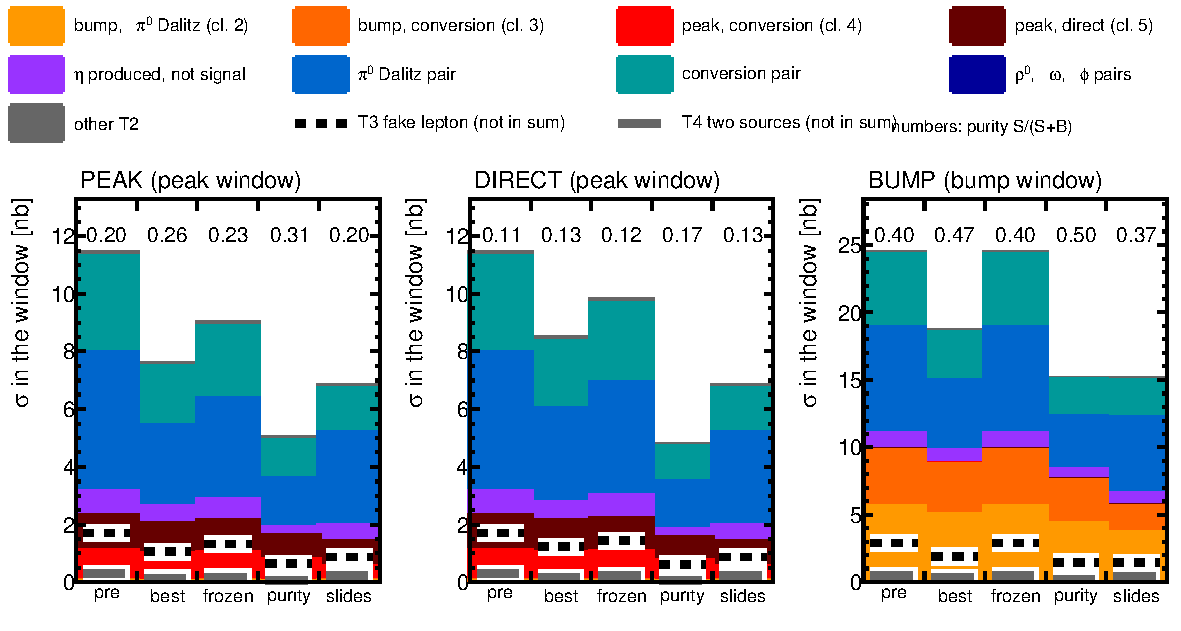
\includegraphics[width=\textwidth]{figs/s5_opt_eta_composition.pdf}
\caption{Content of the target window by group, $\sigma$ in nb, for ``pre'', the best cell, the
frozen cut, the best purity on the plateau and ``slides'' (stacked: T1+T2 groups). T3 (dashed
line) and T4 (dash-dotted line) are drawn at their own level and are not in the stack. Numbers
above the bars: purity $S/(S+B)$.}
\label{fig:s5optcomp}
\end{figure}

\textbf{Split-half check of the optimisation bias.} The rows are split by event group into two
halves (half A = even group number, half B = odd; each half weighted by 2). The search is run on
one half and the chosen cell is evaluated on the other. The bias is $F$(optimising half) $-$
$F$(other half), averaged over both directions, because a single direction also contains the
difference between the halves at fixed cuts (PEAK at ``pre'': $F_A = 51.28$, $F_B = 52.97$).
\begin{center}
\small
\begin{tabular}{@{}l ccc ccc@{}}
\toprule
 & \multicolumn{3}{c}{100 random splits (mean $\pm$ error of the mean)} & \multicolumn{3}{c}{deterministic split (A/B)} \\
target & best cell & freeze rule & purity rule & best cell & freeze rule & purity rule \\
\midrule
PEAK   & $+2.71\pm0.11$\,\% & $+0.68\pm0.09$\,\% & $+1.55\pm0.15$\,\% & $+2.08$\,\% & $+1.77$\,\% & $+0.61$\,\% \\
DIRECT & $+0.75\pm0.05$\,\% & $+0.06\pm0.01$\,\% & $+0.80\pm0.07$\,\% & $+0.37$\,\% & 0.00\,\% & $+1.65$\,\% \\
BUMP   & $+1.10\pm0.07$\,\% & $+0.08\pm0.01$\,\% & $+1.64\pm0.09$\,\% & $+0.65$\,\% & 0.00\,\% & $+1.30$\,\% \\
\bottomrule
\end{tabular}
\end{center}
The gain of the best cell over ``pre'' (PEAK $+7.8$\,\%, DIRECT $+6.0$\,\%, BUMP $+2.8$\,\%) is partly
this bias; the freeze rule reduces it to below 1\,\%. Single directions range from $-7.7$ to
$+9.2$\,\%: this is the noise between halves, set by the std set. The limiting components are
class~4 ($N_{\mathrm{eff}}$ 209 at the frozen PEAK cut; it gives almost all of the 3.0\,\% error of $F$),
the std part of $B$ ($N_{\mathrm{eff}}$ 924) and, for BUMP, the signal itself ($N_{\mathrm{eff}}$ 1739).

\notebox{\textbf{Frozen $\eta$ selections} (\code{plots/eta_sim/}\allowbreak\code{tables/s5_opt_eta_frozen.txt}):
PEAK = pre + $|\Delta z_\pi|<40$\,mm + $\mathrm{MM}_4<2.85$\,\GeVcc; DIRECT = pre + $|\Delta z_\pi|<40$\,mm;
BUMP = pre. \textbf{Caveat for data:} $|\Delta z_\pi|$ needs the $z$ of the pion tracks, which the
compact data rows (\code{ScanEngine.h}) do not have yet. The data-ready alternative on the plateau is
``pre + pions in vertex fit'' ($F/F_{\mathrm{best}}$ = 0.954, 0.962, 0.980). Without CB the
simulation-only optimum may be looser than the data optimum, since the CB and its subtraction
add to the variance and the cuts also reduce the CB.}

%----------------------------------------------------------------------
\subsection{A selection aimed at X17 and its expected limit}
\label{sec:s5x17}
%----------------------------------------------------------------------
\textbf{The X17 line.} In the peak window after ``pre'', the reconstructed \Mee of the X17 rows has
a mean of $17.25\pm0.01$\,\MeVcc and a Gaussian core of $\sigma = 4.04\pm0.01$\,\MeVcc; 93.3\,\% lie
within $\pm2\sigma$. The width depends on the opening angle: 4.5\,\MeVcc for OA$<2^\circ$,
3.3\,\MeVcc for OA$>8^\circ$; the mean moves from 13.6 (OA$<3^\circ$) to 20.3\,\MeVcc
(OA$>8^\circ$), so an OA cut reshapes the line. In \Mfour the X17 rows have mean 546.6\,\MeVcc and
$\sigma = 5.9$\,\MeVcc; 85.7\,\% of them lie in the peak window.

\textbf{Figure of merit.} The expected 90\,\% CL upper limit on
$\mathrm{BR}\equiv\mathrm{BR}(\eta\to\pipi X17)\,\mathrm{BR}(X17\to\ee)$ from counting in a window,
for $\mathrm{BR}=0$:
\begin{equation}
\mathrm{UL} = \sqrt{\mathrm{UL}_{\mathrm{stat}}^2 + \left(1.645\,\sigma_{B,\mathrm{MC}}/s_1\right)^2},
\qquad \mathrm{UL}_{\mathrm{stat}} = s_{\mathrm{up}}(B)/s_1 .
\label{eq:s5ul}
\end{equation}
Here $s_1$ is the number of selected X17 rows per unit BR and $B$ the background rows (T1 without
X17, plus T2), both at \Ldata; $s_{\mathrm{up}}(B)$ is the CLs upper limit on the signal for an
observed count equal to $B$ (continuous Poisson, about $1.645\sqrt{B}$ for large $B$); and
$\sigma_{B,\mathrm{MC}}$ is the simulation (event-group) error of $B$. The second term is there
because a counting analysis takes $B$ from this simulation. $\mathrm{UL}_{\mathrm{stat}}$ alone is
the limit with the background known exactly: a statistical limit only.

\textbf{Two versions.} The first optimisation (v1, used by the blind test of
Sect.~\ref{sec:s5blind}) used $\mathrm{UL}_{\mathrm{stat}}$ and also optimised the edges of the
\Mfour window. A review found two problems: the MC error of $B$ ($\pm307$ rows) is larger than
the statistical term, and the \Mfour window was to stay fixed for all parts of the study. The
optimisation was therefore repeated (v2) with Eq.~(\ref{eq:s5ul}) and the fixed peak window.
Method: coordinate descent over \Mee window, OA (lower and upper), $\alpha_{\mathrm{lab}}$,
\Mpipi (lower and upper), $\alpha_\eta$ and pions in the vertex fit; in each step the loosest value
within 2\,\% of the step minimum is taken. Two different starting points end at the same optimum.

\begin{table}[H]
\centering
\caption{X17 selections after ``pre''. Rows at $\Ldata = 6080.5\,\nbinv$ (UNCONFIRMED). UL in
units of $10^{-6}$; ``shape'': binned likelihood of \Mee 2--62\,\MeVcc in the \Mfour window with a
Gaussian X17 line (background shape from the simulation, normalisation known or free).
$Z$: Asimov significance for $\mathrm{BR}=10^{-5}$ with $B$ known.}
\label{tab:s5x17}
\small
\begin{tabularx}{\textwidth}{@{}L >{\raggedright\arraybackslash}p{4.4cm} >{\raggedright\arraybackslash}p{4.4cm}@{}}
\toprule
 & v1 (blind test) & v2 (frozen) \\
\midrule
cuts in addition to ``pre'' & \Mfour 0.5330--0.5555, \Mee 13.0--26.5, pions in vertex fit
                            & \Mfour 0.5333--0.5587, \Mee 15.5--24.5, pions in vertex fit \\
X17 rows per unit BR, $s_1$  & $2.727\times10^{7}$ & $2.127\times10^{7}$ \\
X17 rows at $\mathrm{BR}=10^{-5}$ & 272.7 & 212.7 \\
background $B$ [nb] ($N_{\mathrm{eff}}$) & $1.333\pm0.051$ (696) & $0.878\pm0.039$ (501) \\
background rows $B\pm\sigma_{B,\mathrm{MC}}$ & $8108\pm307$ & $5342\pm239$ \\
$\mathrm{UL}_{\mathrm{stat}}$ (B known exactly) & 5.48 & 5.71 \\
$\mathrm{UL}$, Eq.~(\ref{eq:s5ul}) (with the MC error of $B$) & 19.3 & 19.3 \\
shape, $B$ known / normalisation free & 4.85 / 5.40 & 4.96 / 5.54 \\
$Z$($\mathrm{BR}=10^{-5}$), $B$ known / with $\sigma_{B,\mathrm{MC}}$ & 3.01 / 0.85 & 2.89 / 0.85 \\
\bottomrule
\end{tabularx}
\end{table}

\textbf{Results} (Table~\ref{tab:s5x17}, Fig.~\ref{fig:s5x17shape}).
\begin{itemize}
\item \textbf{The MC error of the background sets the limit.} With the MC term the expected limit is
      $1.93\times10^{-5}$ for both selections, 3.4--3.5 times $\mathrm{UL}_{\mathrm{stat}}$. The
      re-optimisation gains nothing: the v1 cuts give $1.933\times10^{-5}$, the v2 cuts
      $1.931\times10^{-5}$. ``slides'' with the same \Mee window gives $2.15\times10^{-5}$.
\item \textbf{Where the MC error comes from.} At the v2 optimum the variance of $B$ comes from
      $G_{\pi^0\mathrm{D}}$ (60\,\%; lep set, $N_{\mathrm{eff}}$ 313), $G_{\mathrm{conv}}$ (24\,\%; 19 std
      rows, $N_{\mathrm{eff}}$ 18) and $G_\eta$ (12\,\%; $N_{\mathrm{eff}}$ 29). One std row stands for 27.5
      expected data rows.
\item \textbf{Cuts.} The \Mee window keeps 0.62 of X17 and 0.094 of $B$; the pion-vertex cut keeps
      0.93 of X17 and 0.82 of $B$. OA, $\alpha_{\mathrm{lab}}$, \Mpipi and $\alpha_\eta$ cuts do not
      lower the limit: at \Mee 12--22\,\MeVcc the OA medians of X17 (4.9$^\circ$), the direct decay
      (4.6$^\circ$) and $G_{\pi^0\mathrm{D}}$ (5.2$^\circ$) are about the same.
\item \textbf{Composition of $B$} (v1): $G_{\pi^0\mathrm{D}}$ 0.56, direct decay (class 5) 0.18,
      $G_{\mathrm{conv}}$ 0.12, $G_\eta$ 0.08, class 4 0.03. The direct decay is an irreducible
      background under the line.
\item \textbf{Split halves} (v2 figure of merit): the optimum of half A gives 28.1 on A and 30.2 on
      B, that of half B 24.4 and 28.1 (in $10^{-6}$; each half has a $\sqrt2$ larger MC error). The
      bias is 7--15\,\%: with the MC term the figure of merit is itself noisy, and the optimum
      (\Mee 13--27.5 on half A, 15.5--23.5 on half B) is not better determined than in v1.
\end{itemize}

\begin{figure}[H]
\centering
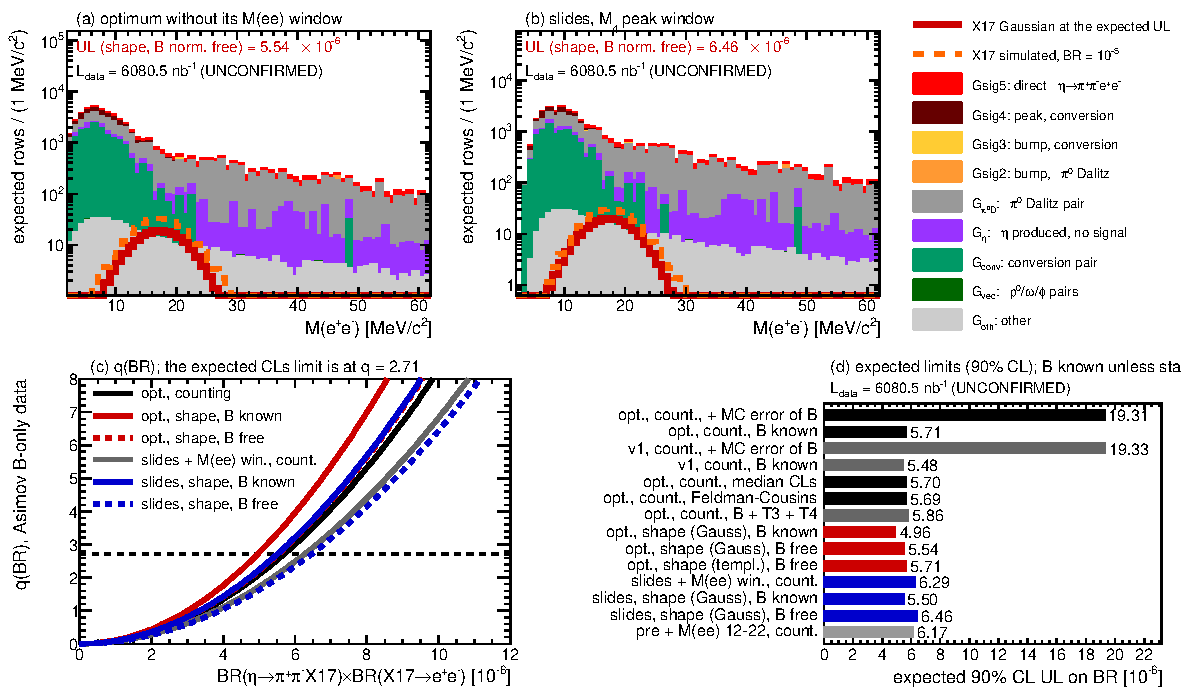
\includegraphics[width=\textwidth]{figs/s5_opt_x17_shape.pdf}
\caption{X17 search, expected rows at $\Ldata = 6080.5\,\nbinv$ (UNCONFIRMED). (a) \Mee at the v2
optimum without its \Mee window, stacked background groups, X17 as a Gaussian at the expected limit
of the shape fit and as the simulated template at $\mathrm{BR}=10^{-5}$. (b) The same for
``slides''. (c) Test statistic $q(\mathrm{BR})$ on Asimov background-only data; the expected
CLs limit is at $q = 2.71$. (d) Expected 90\,\% CL limits; ``B known'' ignores the MC error of $B$.}
\label{fig:s5x17shape}
\end{figure}

\notebox{\textbf{Frozen X17 selection v2} (\code{plots/eta_sim/}\allowbreak\code{tables/s5_opt_x17_frozen.txt}; v1 kept in
\code{s5_opt_x17_frozen_v1.txt}): pre + peak window + $15.5\le\Mee<24.5$\,\MeVcc + both pions in
the vertex fit. Expected 90\,\% CL limit by counting $1.9\times10^{-5}$ including the MC error of
the background; $5.7\times10^{-6}$ if the background were known exactly. These numbers assume
$\Ldata = 6080.5\,\nbinv$ (UNCONFIRMED), no CB, the SMASH background and phase space for X17.}

%----------------------------------------------------------------------
\subsection{Blind test of the signal extraction and of the X17 search}
\label{sec:s5blind}
%----------------------------------------------------------------------
The extraction methods planned for the data were tested on simulated pseudo-data whose true
content was hidden from the analyst until the procedure was frozen.

\textbf{Preparation.}
\begin{enumerate}
\item \textbf{Split.} The rows are split by event group: half A (even group number) gives the
      templates, half B (odd) gives the pseudo-data. Every row of an event goes to the same half.
\item \textbf{Templates}: half A with weights $\times2$, histograms of \Mfour (1\,\MeVcc bins) per
      component and selection (PEAK, DIRECT, BUMP of Sect.~\ref{sec:s5opt} and the v1 X17 selection),
      exact window sums, and \Mee and $\Mfour\times\Mee$ for X17.
\item \textbf{$\eta$ pseudo-data}: 200 toys at $L_{\mathrm{toy}} = \Lsim/2 = 110.525\,\nbinv$ from a
      Poisson bootstrap of half B per event group. An event with largest row weight $w_g$ enters
      $n\sim\mathrm{Poisson}(w_g)$ times; in each copy one uniform $u$ is drawn and each row with
      $w_r/w_g>u$ is kept, so that every row has the expected multiplicity $w_r$. Only T1+T2 rows
      are used. A check with 4000 toys gave toy variance / predicted variance = 0.95--1.06; the sum
      of the squared pulls of the variances over the 21 regions was 36.8. Repeated with eight further
      random seeds, this sum is 9.1--35.7, on average $20.7\pm10.1$ over all nine runs (21 expected; the
      spread is wider than for 21 independent entries because the selections share rows), and the
      variance ratio stays within 0.94--1.06: the bootstrap reproduces the variances, the value 36.8 is
      a fluctuation.
\item \textbf{X17 pseudo-data}: 1500 toys at \Ldata (UNCONFIRMED), parametric: in each cell of
      $\Mfour\times\Mee$ signal and background are drawn as Poisson numbers around the half-B
      expectation ($\times2\times\Ldata/\Lsim$). BR $\in\{0, 1, 3, 10, 30\}\times10^{-6}$, 300 toys
      each, shuffled, with random ids.
\item \textbf{Sealed key}: true rows per toy, group and region; the expectation of half B per
      toy, called $\mu$, is the quantity a measurement would estimate.
\end{enumerate}
For the weight rules~v2 the $\eta$ and X17 toys were drawn again with the same seed. Because
the weights changed, the random draws differ from those of rules~v1, so the biases and pulls
moved within their statistical errors (by up to 2.3 standard deviations).

\textbf{Methods} (frozen before any yield was computed on the pseudo-data). Peak yield: M1 =
Gaussian (fixed at 0.5460\,\GeVcc, 6.7\,\MeVcc) + second-order polynomial, calibrated with the
response to the half-A peak template; M2 = template fit (free normalisations of peak, bump and
background templates, binned Poisson likelihood with the template variance added); M2b = M2
with the background split into $G_\eta$ and the rest; M2d = M2 with the peak split into class 5
(free) and class 4 (constrained to its half-A value $\pm$ its MC error); M3 = linear side bands
(7.8\,\MeVcc on each side) with the signal leakage $\lambda$ into the side bands corrected,
$S = [N_{\mathrm{win}} - (N_L+N_U)/2\cdot25.4/7.8]/(1-\lambda)$; M3c = M3 with the curvature of
the background taken from half A. Bump yield: B1 = bifurcated Gaussian + $\eta$ Gaussian +
polynomial; B2 = the bump of M2; B3 = edge step in \Mfour; B4 = side band 0.5665--0.70 with
the background shape from half A. Direct yield: M2d, and D5 = split at $\Mee = 10$\,\MeVcc with a
$2\times2$ unfolding. X17: X1 = fit of \Mee in the window with free normalisations of the direct
decay and the rest; X2 = X1 with the raw half-A template; X3 = X1 on 8--40\,\MeVcc; X4 = X1 with
the direct-decay normalisation constrained to $1\pm0.10$; X5 = counting with $B$ from half A.
X4 and X5 were added after the X1 results were seen (declared, before their own results). An
example toy with the fits is shown in Fig.~\ref{fig:s5toy}.

\begin{figure}[H]
\centering
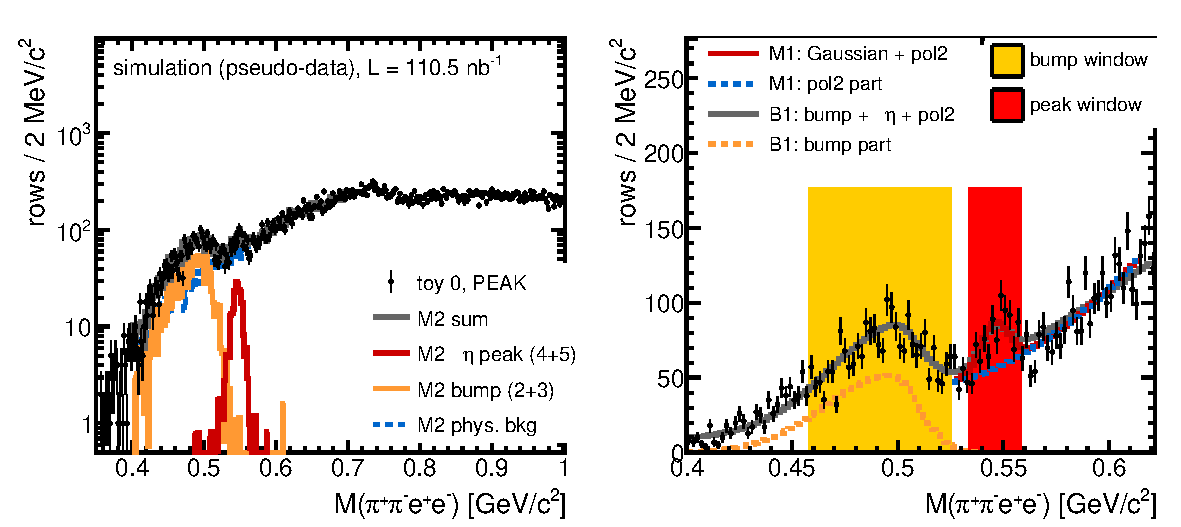
\includegraphics[width=\textwidth]{figs/s5_blind_ana_toy0_PEAK.pdf}
\caption{One $\eta$ toy (pseudo-data, $L = 110.5\,\nbinv$, PEAK selection). Left: \Mfour with
the components of the template fit M2. Right: zoom with the Gaussian + polynomial fit M1 and the
bump fit B1, with the bump and peak windows.}
\label{fig:s5toy}
\end{figure}

\textbf{What a bias means here.} The templates (half A) and the pseudo-data (half B) are two
statistically independent copies of the same model. The truth of half B differs from half A by
MC fluctuations: peak (PEAK selection) $241.4$ against $224.1\pm10.3$ rows (+7.7\,\%), bump (BUMP)
1095.6 against $1046.1\pm35.7$ (+4.7\,\%), class 5 (DIRECT) 128.88 against $128.00\pm0.48$, class 4
(DIRECT) 118.5 against $106.2\pm10.5$ (+11.5\,\%). All toys share this difference. A method bias
can therefore be resolved only beyond the common MC error, which is $\pm$11--15\,\% for the peak and
$\pm$4.5--5\,\% for the bump.

\begin{table}[H]
\centering
\caption{Blind test, $\eta$ yields (200 toys). Bias = $\langle Y\rangle - \mu$ with the error of the
mean over toys and the common MC error (template and parent sample). Pull = $(Y-\mu)/\sigma_{\mathrm{tot}}$
with the error quoted by the analyst (mean/rms). Coverage: fraction of toys with
$|Y-\mu|\le\sigma_{\mathrm{tot}}$ (nominal 0.683).}
\label{tab:s5blind}
\footnotesize
\setlength{\tabcolsep}{4pt}
\begin{tabular}{@{}l l r r c c@{}}
\toprule
yield, selection ($\mu$) & method & bias [rows] & relative & pull & coverage \\
\midrule
peak, PEAK (241.4)  & M1 Gauss + pol2   & $+7.4\pm2.9\pm31.3$  & $+3.1$\,\%  & $+0.17$ / 0.96 & 0.72 \\
                    & M2 template fit   & $+3.4\pm2.0\pm27.5$  & $+1.4$\,\%  & $+0.08$ / 0.80 & 0.77 \\
                    & M2b               & $+10.4\pm2.2\pm30.6$ & $+4.3$\,\%  & $+0.26$ / 0.82 & 0.74 \\
                    & M3 side bands     & $-51.0\pm3.9\pm45.3$ & $-21.1$\,\% & $-0.86$ / 0.93 & 0.53 \\
                    & M3c               & $-124.5\pm3.9\pm56.9$ & $-51.6$\,\% & $-1.82$ / 0.80 & 0.16 \\
\midrule
bump, BUMP (1095.6) & B4 side band & $+42.3\pm3.9\pm54.9$ & $+3.9$\,\% & $+0.61$ / 0.79 & 0.66 \\
                    & M2 template fit   & $+84.5\pm3.4\pm49.7$ & $+7.7$\,\%  & $+1.34$ / 0.76 & 0.31 \\
                    & B1 parametric     & $+59.0\pm7.1\pm78.6$ & $+5.4$\,\%  & $+0.56$ / 0.96 & 0.66 \\
                    & B3 edge step      & $+13.8\pm13.3\pm171.5$ & $+1.3$\,\% & $+0.01$ / 0.86 & 0.76 \\
\midrule
direct, DIRECT (128.9) & M2d (cl.\ 4 constr.) & $+26.6\pm2.2\pm31.0$ & $+20.6$\,\% & $+0.68$ / 0.79 & 0.62 \\
                    & D5 (\Mee split)   & $+40.5\pm3.9\pm39.3$ & $+31.4$\,\% & $+0.70$ / 0.96 & 0.61 \\
\bottomrule
\end{tabular}
\end{table}

\textbf{$\eta$ results} (Table~\ref{tab:s5blind}, Fig.~\ref{fig:s5bias}).
\begin{itemize}
\item \textbf{Peak.} The template fit M2 and the calibrated Gaussian fit M1 find the peak within
      +1 to +6\,\% in all three selections, well inside the common MC error. Per toy they differ by
      about 12\,\% (rms 29 rows), so a difference of that size between them in data is normal.
      M2b is 3--8\,\% above M2 every time.
\item \textbf{Linear side bands (M3) lose the peak}, because the background is convex under it and
      17\,\% of the signal leaks into the side bands. Two independent realisations of the MC noise
      measure this: the half-B toys give $-21$\,\%, $-13$\,\%, $-16$\,\% and the exact half-A sums
      (Asimov) $-40$\,\%, $-43$\,\%, $-46$\,\% (PEAK, DIRECT, BUMP); the mean is about $-30\pm14$\,\%.
      The MC-calibrated version M3c over-corrects ($-44$ to $-52$\,\%), because the curvature from
      the simulation is itself noisy.
\item \textbf{Bump.} B4 is closest (+3 to +4\,\%); the template fit agrees within 3--8\,\%; the
      parametric fit B1 comes out 5--10\,\% high; the edge step B3 is unbiased but has 15--17\,\%
      statistical error.
\item \textbf{Direct decay alone.} \Mfour cannot separate class 5 from class 4. M2d gives
      class 4 = 105.4 (truth 118.5) and therefore class 5 too high by the same amount
      ($26.6 = 13.5 + 13.1$ rows). The split is limited by the simulation statistics of the
      conversion peak ($N_{\mathrm{eff}}\approx100$ in a half).
\item \textbf{Errors.} The event-group errors describe the spread of the toys: the ratio rms/error
      is 0.93--1.08 for M1, M3, B1, B3 and D5 and 0.90--1.06 for the template fits and B4, so the
      errors are adequate. The common MC error is not in the per-toy error and must be added.
\end{itemize}

\begin{figure}[H]
\centering
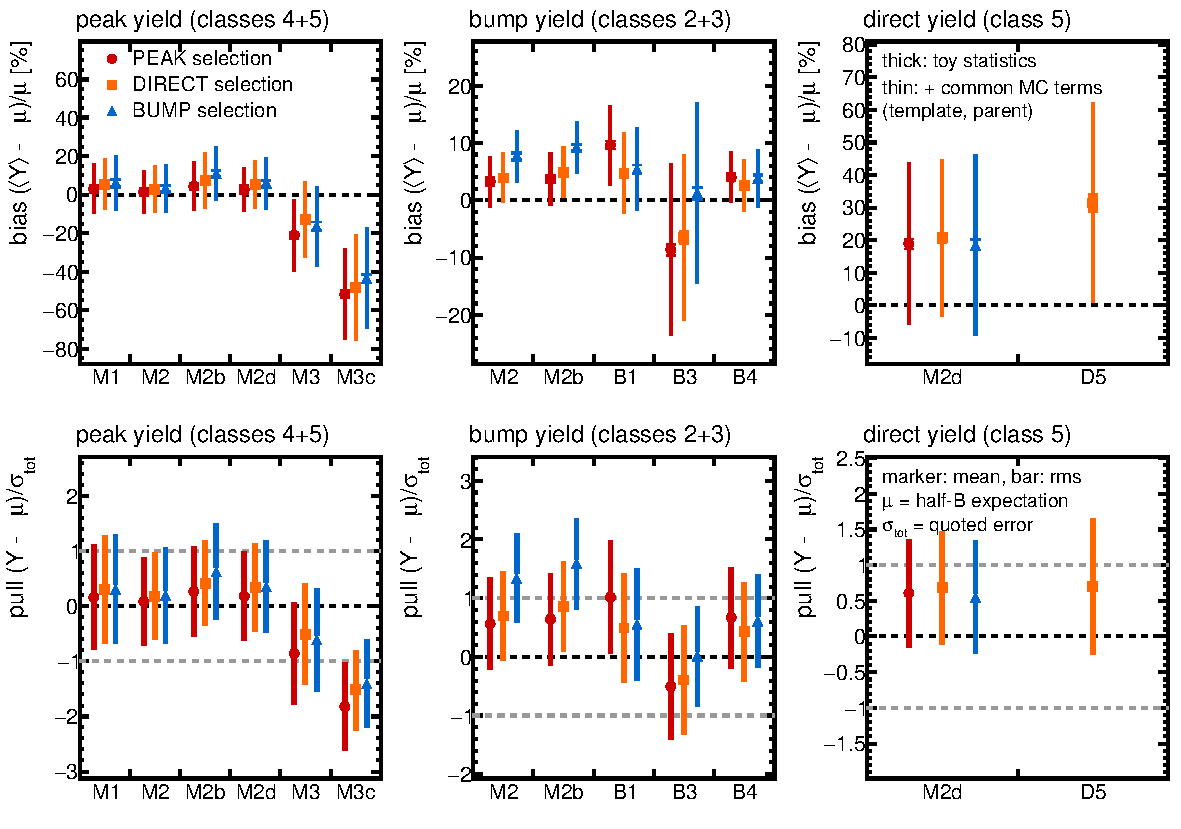
\includegraphics[width=\textwidth]{figs/s5_blind_eval_eta_bias.pdf}
\caption{Blind test, $\eta$ yields. Top: relative bias $(\langle Y\rangle-\mu)/\mu$ per method and
selection; thick bars: toy statistics, thin bars: including the common MC terms. Bottom: pull
$(Y-\mu)/\sigma_{\mathrm{tot}}$, marker = mean, bar = rms.}
\label{fig:s5bias}
\end{figure}

\textbf{X17 results} (Table~\ref{tab:s5blindx}, Figs.~\ref{fig:s5side} and~\ref{fig:s5x17lin}).
Each std row of half B stands for about 55 expected data rows. The background of every X17 toy
is therefore the unsmoothed half-B content, with single-bin spikes of 50--200 rows that all toys
share and that differ from half A (Fig.~\ref{fig:s5side}).
\begin{itemize}
\item Every estimator follows the injected BR with a slope of 0.98--1.02.
\item The zero point is shifted, by the same amount in all toys: it is set by how well the
      background under the line is known. Counting with the half-A background (X5) closes exactly:
      the predicted shift $(B_B-B_A)/s_1 = (7947.8-8268.2)/2.725\times10^{7} = -11.76\times10^{-6}$
      is measured as $-11.66\pm0.19\times10^{-6}$ at $\mathrm{BR}=0$.
\item Only estimators whose error contains this background uncertainty give valid limits (X1, X4,
      X5 cover the true BR at every BR). Their median limits at $\mathrm{BR}=0$ are
      $2.1$--$6.2\times10^{-5}$, 4--11 times the $\mathrm{UL}_{\mathrm{stat}}$ of v1, and consistent
      with the $1.9\times10^{-5}$ of Eq.~(\ref{eq:s5ul}).
\item Estimators with a small error (X2, X3, X1 with the statistical error only) exclude the true
      BR. No estimator claimed a $3\sigma$ signal at $\mathrm{BR}=0$, but only because the common shift
      happens to be negative: with the opposite sign X2 and X3 would claim one in 100\,\% and 98\,\%
      of the toys.
\end{itemize}

\begin{table}[H]
\centering
\caption{Blind test, X17 (1500 toys at $\Ldata = 6080.5\,\nbinv$, UNCONFIRMED; BR in $10^{-6}$).
Offset: mean extracted BR at injected $\mathrm{BR}=0$. Coverage: fraction of toys whose UL is above
the injected BR. X1--X3 were frozen; X4 (X1 with the direct-decay normalisation $a_D$ constrained) and X5
(counting) were added after the freeze.}
\label{tab:s5blindx}
\footnotesize
\setlength{\tabcolsep}{4pt}
\begin{tabular}{@{}l c c c c@{}}
\toprule
estimator & offset at 0 & slope & median UL at 0 (16--84\,\%) & UL coverage at 0 / 3 / 10 / 30 \\
\midrule
X1 window fit         & $-72.7\pm0.5$ & $1.004\pm0.021$ & 31.2 (28.2--34.4) & 1.00 / 1.00 / 1.00 / 0.99 \\
X2 raw template       & $-72.4\pm0.6$ & $0.977\pm0.024$ & 2.5 (2.1--3.3)    & 1.00 / 0.34 / 0.00 / 0.00 \\
X3 8--40\,\MeVcc     & $-74.9\pm0.3$ & $0.996\pm0.011$ & 12.7 (11.8--13.5) & 1.00 / 1.00 / 1.00 / 0.00 \\
X4 X1, $a_D = 1\pm0.1$ & $-1.1\pm0.4$  & $1.016\pm0.018$ & 61.8 (57.3--67.3) & 1.00 at all BR \\
X5 counting                   & $-11.7\pm0.2$ & $0.999\pm0.008$ & 21.1 (19.7--22.7) & 1.00 at all BR \\
\bottomrule
\end{tabular}
\end{table}

\begin{figure}[H]
\centering
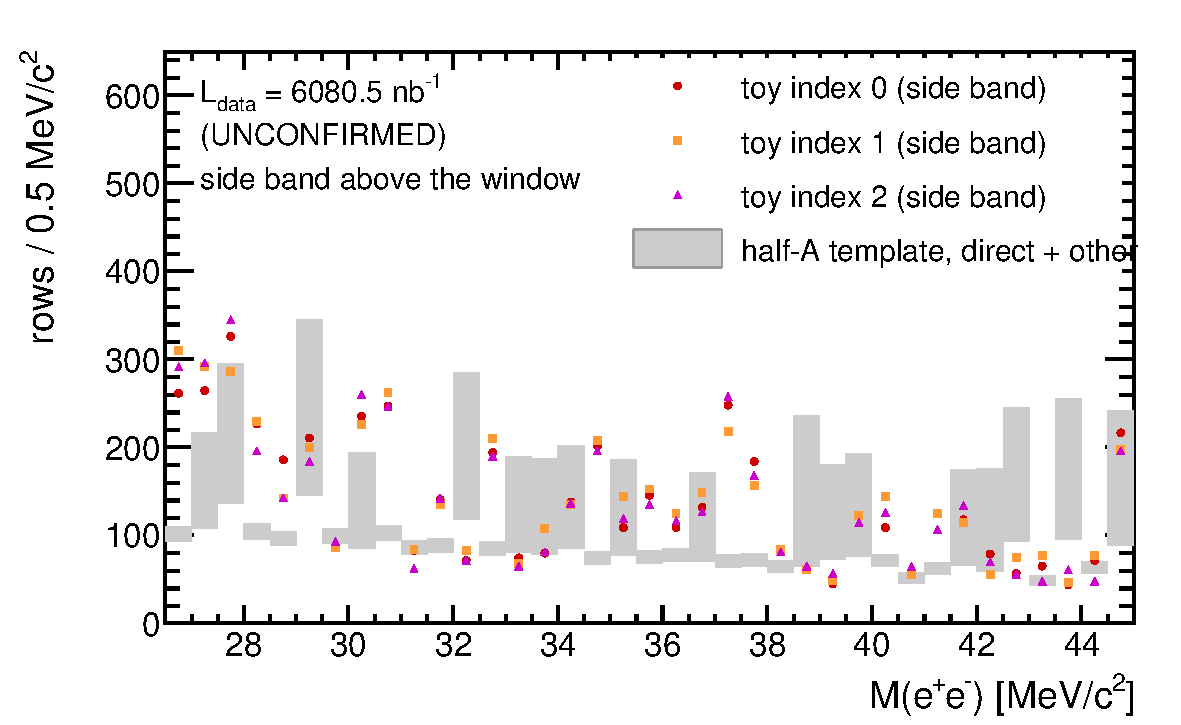
\includegraphics[width=0.75\textwidth]{figs/s5_blind_ana_x17_sideband.pdf}
\caption{\Mee side band (above the X17 window) of three X17 toys against the half-A template
(grey boxes). All toys show the same spikes, which come from single heavy rows of half B.
$\Ldata = 6080.5\,\nbinv$ (UNCONFIRMED).}
\label{fig:s5side}
\end{figure}

\begin{figure}[H]
\centering
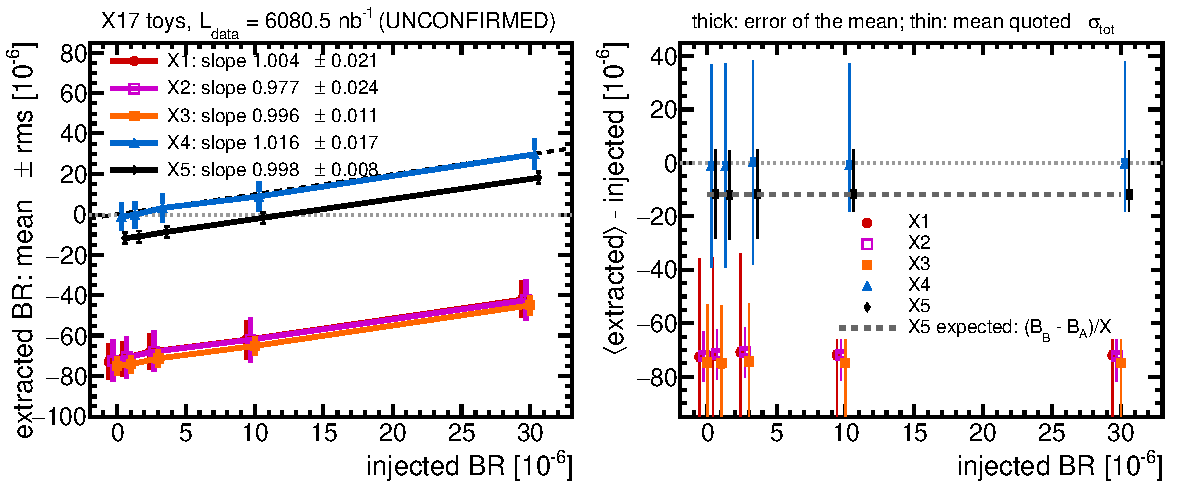
\includegraphics[width=\textwidth]{figs/s5_blind_eval_x17_linearity.pdf}
\caption{Blind test, X17. Left: extracted against injected BR (mean $\pm$ rms over 300 toys) with
straight-line fits. Right: mean offset; thick bars: error of the mean, thin bars: mean quoted
error. Dotted: the offset predicted for X5. $\Ldata = 6080.5\,\nbinv$ (UNCONFIRMED).}
\label{fig:s5x17lin}
\end{figure}

\textbf{Limits of this test.} The test is a closure test inside one model. It does not show how
the methods behave in data.
\begin{itemize}
\item Templates and pseudo-data come from the same SMASH model; there is no CB and no data/SMASH
      shape difference (0.87--1.36 above 0.56\,\GeVcc in earlier comparisons). Template fits are
      favoured by construction. $L_{\mathrm{toy}}$ is 55 times below \Ldata.
\item \textbf{The test was not blind by construction.} The frozen tables that the analyst read
      contain full-sample (A+B) numbers; together with the half-A templates they give the half-B
      truth (for example the PEAK yield 241.4 and the X17 background of half B). No sign was found
      that these numbers were used, and the sealed key was not read before the results were
      written, but the leak was possible.
\item The bootstrap repeats identical rows; how often a row recurs across toys reveals its set and
      therefore class 4 (std) against class 5 ($\eta$ set). This was not exploited, but it is a
      second possible leak.
\item The X17 part used the v1 selection, whose \Mfour window was optimised (partly on a step of
      4 to 8 std rows); the fixed window raises $\mathrm{UL}_{\mathrm{stat}}$ by 3\,\%.
\end{itemize}

%----------------------------------------------------------------------
\subsection{What this means for the data analysis}
\label{sec:s5data}
%----------------------------------------------------------------------
\begin{enumerate}
\item \textbf{Cuts.} In the simulation the four $\eta$-selection cuts remove background outside the
      windows but do not improve the windows themselves; OA$>2^\circ$ and $\alpha_\eta>140^\circ$ cost
      signal (conversions, bump). Their use in data must be justified by the CB and checked there.
      The pion-vertex cuts are the only ones with a gain inside the windows (4--6\,\%); the frozen
      PEAK and DIRECT cuts need the pion track $z$ in the data compact rows, otherwise ``pre + pions
      in vertex fit'' is the alternative.
\item \textbf{Peak extraction.} Template fit (M2) and Gaussian + polynomial with calibration (M1)
      close within a few per cent in simulation; a difference of about 12\,\% between them is normal.
      Linear side bands under the peak lose 20--45\,\% and should not be used.
\item \textbf{Bump.} Side band with the simulated background shape (B4) and template fit; the
      parametric fit tends to be high.
\item \textbf{Direct decay alone.} The split of the peak into class 5 and class 4 is limited by the
      307 std rows of class 4; the quoted error must include the simulation statistics.
\item \textbf{Simulation statistics.} The std set limits the bump and conversion templates
      ($N_{\mathrm{eff}}$ 270--1332) and the X17 background. The common MC error must be added to every
      yield.
\item \textbf{X17.} With the background taken from this simulation the expected limit is about
      $2\times10^{-5}$ (at $\Ldata$ UNCONFIRMED), set by the simulation statistics of the background;
      $5.7\times10^{-6}$ would need the background known exactly. Any X17 estimate must carry the
      background uncertainty in its error. A larger std production or a background determined from
      data side bands would be needed to approach the statistical limit.
\end{enumerate}

\tipbox{\textbf{Open points of this section.} (i) $\Ldata$ is UNCONFIRMED. (ii) The absolute
efficiencies rest on $N_{\mathrm{direct}} = 100\times1\,181\,801$ (representativeness of the 1000
generator files UNVERIFIED). (iii) The X17 \Mpipi distribution and decay angle are assumed
(phase space, isotropic). (iv) The blind test should be repeated with cut definitions only, with
hidden per-toy signal scales and with pseudo-data that do not repeat identical rows; a version with
a CB-like component and a reweighted background shape would test the methods closer to data.
(v) The pion-vertex variables were not compared between simulation and data. (vi) The beam
energy (4530 in the analysis, 4500\,MeV in SMASH) does not affect \Mfour, \Mee and \Mpipi, but does
affect $\mathrm{MM}_4$.}
